\documentclass[12pt,titlepage,a4paper]{report}
\usepackage[margin=1in]{geometry}
\usepackage{graphicx,amsmath,blindtext,minted}

%% Variables definition
\newcommand{\vSubject}{Project Implementation Plan}
\newcommand{\vSubtitle}{Room Tenant System}
\newcommand{\vName}{Muhammad Baihaqi Aulia Asy'ari}
\newcommand{\vNIM}{2241720145}
\newcommand{\vClass}{2I}
\newcommand{\vGroup}{Group 4}
\newcommand{\vDepartment}{Information Technology}
\newcommand{\vStudyProgram}{D4 Informatics Engineering}

%% [START] Tikz related stuff
\usepackage{tikz}
\usetikzlibrary{svg.path,calc,shapes.geometric,shapes.misc}
\tikzstyle{terminator} = [rectangle, draw, text centered, rounded corners = 1em, minimum height=2em]
\tikzstyle{preparation} = [chamfered rectangle, chamfered rectangle sep=0.75em, draw, text centered, minimum height = 2em]
\tikzstyle{process} = [rectangle, draw, text centered, minimum height=2em]
\tikzstyle{decision} = [diamond, aspect=2, draw, text centered, minimum height=2em]
\tikzstyle{data}=[trapezium, draw, text centered, trapezium left angle=60, trapezium right angle=120, minimum height=2em]
\tikzstyle{connector} = [line width=0.25mm,->]
%% [END] Tikz related stuff

%% [START] Fancy header related stuff
\usepackage{fancyhdr}
\pagestyle{fancy}
\fancyhf{}
\setlength{\headheight}{15pt} % compensate fancyhdr style
\fancyhead{}
\fancyfoot{}
\fancyfoot[L]{\thepage}
\fancyfoot[R]{\textit{\vSubject - \vSubtitle}}
\renewcommand{\footrulewidth}{0.4pt}% default is 0pt, overline for footer

\fancypagestyle{plain}{
    \fancyhf{}
    \setlength{\headheight}{15pt} % compensate fancyhdr style
    \fancyhead{}
    \fancyfoot{}
    \fancyfoot[L]{\thepage}
    \fancyfoot[R]{\textit{\vSubject - \vSubtitle}}
    \renewcommand{\footrulewidth}{0.4pt}% default is 0pt, overline for footer
}
%% [END] Fancy header related stuff

%% [START] Custom tabular command related stuff
\usepackage{tabularx}
\newcommand{\details}[2]{
    #1 & #2  \\
}
%% [END] Custom tabular command related stuff

%% [START] Figure related stuff
\newcommand{\image}[3][1]{
    \begin{figure}[h]
        \centering
        \includegraphics[#1]{#2}
        \caption{#3}
        \label{#3}
    \end{figure}
}
%% [END] Figure related stuff

%%
\usepackage{pgf-umlcd}

\renewcommand{\umldrawcolor}{black}
\renewcommand{\umlfillcolor}{white}
%%

%% [BEGIN] Custom enumerator
\usepackage{enumitem}
%% [END] Custom enumerator

%% [BEGIN] Paragraph indent
\usepackage{indentfirst}
%% [END] Paragraph indent

\renewcommand\thesection{\Alph{section}.}
\renewcommand\thesubsection{\alph{subsection}.}

\usepackage{rotating}

%% [BEGIN] URL
\usepackage{hyperref}
\hypersetup{
    colorlinks=true,
    linkcolor=blue,
    filecolor=magenta,      
    urlcolor=cyan,
    pdftitle={Overleaf Example},
    pdfpagemode=FullScreen,
    }

\urlstyle{same}
%% [END] URL

\begin{document}
\begin{titlepage}
    \centering
    \vfill
    {\bfseries\LARGE
        \vSubject\\
        \vskip0.25cm
        \vSubtitle
    }
    \vfill
    
\includegraphics[width=6cm]{images/polinema-logo.png}
    \vfill
    {
        \textbf{\vGroup} \\
        \vspace{0.5cm}
        \textbf{Group Members}\\
        \vspace{0.5cm}
        \begin{tabular}{l l}
            Dicha Zelianivan Arkana         & \textbf{2241720002} \\
            Davis Maulana Hermanto          & \textbf{2241720255} \\
            Muhammad Baihaqi Aulia Asy'ari  & \textbf{2241720145} \\
            Sri Kresna Maha Dewa            & \textbf{2241720244} \\
            Steven Christian Susanto        & \textbf{2241720003} \\
            Yanuar Thaif Chalil Candra      & \textbf{2241720004} \\            
        \end{tabular}
        \vskip0.5cm
        \textbf{Class}\\
        \vClass\\
        \vskip0.5cm
        \textbf{Department}\\
        \vDepartment\\
        \vskip0.5cm
        \textbf{Study Program}\\
        \vStudyProgram
    }
\end{titlepage}

\tableofcontents

\newpage

\chapter{Project Description}
    \section{Project Name}
    Information Technology Room Tenant System
    \section{Bussiness Needs}
    In the Informatics Department, There is a standard operating procedure to borrow a room for events such as seminars, workshops, etc. Despite having the standard operating procedure, the procedure itself is deemed unnecessarily complicated and tedious. This app is aimed to streamline the process of borrowing rooms in the JTI building.
    \section{Product Perspective}
    This app is made to reduce the amount of paperwork and administrative workload being done manually. The staff and faculty of JTI will use the app to manage the rooms and the events. The students will also use the app to book the rooms for their events. This app will also ensure the borrower's reserved room isn't being overridden by any third party or will clarify why the reserved room is being overridden if anything happened that has higher priority than the borrower's event. This app aims for bureaucracy transparency to minimize miscommunication and misunderstanding.
    \section{Project Scope}
    \begin{enumerate}[label=\alph*.]
        \item In Scope
        \begin{enumerate}[label=\roman*.]
            \item The project is a web app that can be accessed by the admins of the inventory using a web browser.
            \item The app should have a basic authentication feature to ensure that only the authorized users can access the app.
            \item The app should be able to provide a way for the admins to manage the inventory, such as adding, removing, and updating the room and event data.
            \item The admin and student should be able to see the list of rooms and events.
            \item The app should be able to provide a way for the admins to manage the users, such as adding, removing, and updating the users.
            \item The app should provide a way for students to borrow a room from the list. Each room can only be borrowed for a certain amount of time.
            \item The admins should be able to see the history of the room borrowings.
            \item The app should never give an invalid state such as the start of the borrowing time is after the end of the borrowing time.
        \end{enumerate}
        \item Out of Scope
        \begin{enumerate}[label=\roman*.]
            \item Integration with other systems, such as the university's student information system for Single Sign-On (SSO).
        \end{enumerate}
    \end{enumerate}
    \section{Project Team}
    \begin{tabular}{|l|l|}
        \hline
        Members & Role \\
        \hline
        Dicha Zelianivan Arkana & Fullstack Developer \\
        \hline
        Davis Maulana Hermanto & Frontend Developer \\
        \hline
        Muhammad Baihaqi Aulia Asy'ari & System Analyst \\
        \hline
        Sri Kresna Maha Dewa & UI\slash UX Designer \\
        \hline
        Steven Christian Susanto & Frontend Developer \\
        \hline
        Yanuar Thaif Chalil Candra & UI\slash UX Designer \\
        \hline
    \end{tabular}
    \section{Project Scheduling}
    \begin{turn}{90}
        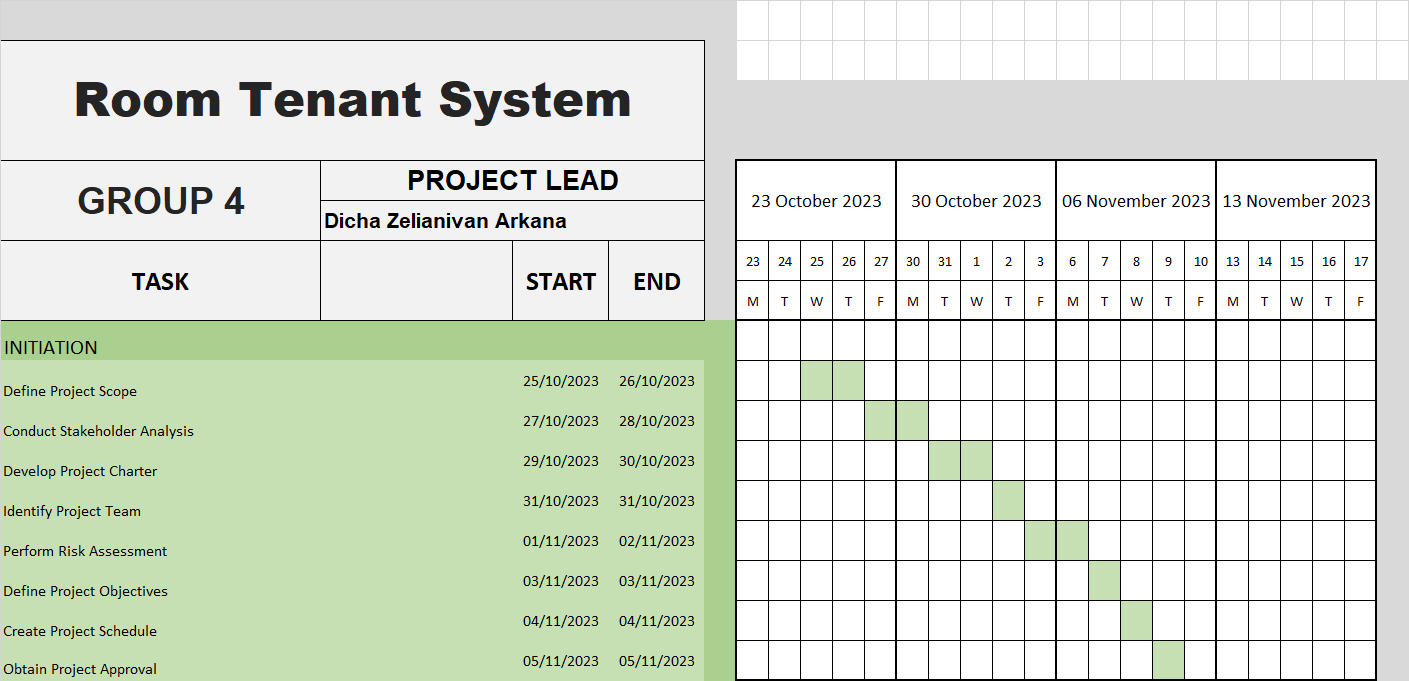
\includegraphics[width=.95\textheight]{images/figures/gant-Init.png}
    \end{turn}\\
    \begin{turn}{90}
        \includegraphics[width=\textheight]{images/figures/gant-Plan.png}
    \end{turn}\\
    \begin{turn}{90}
        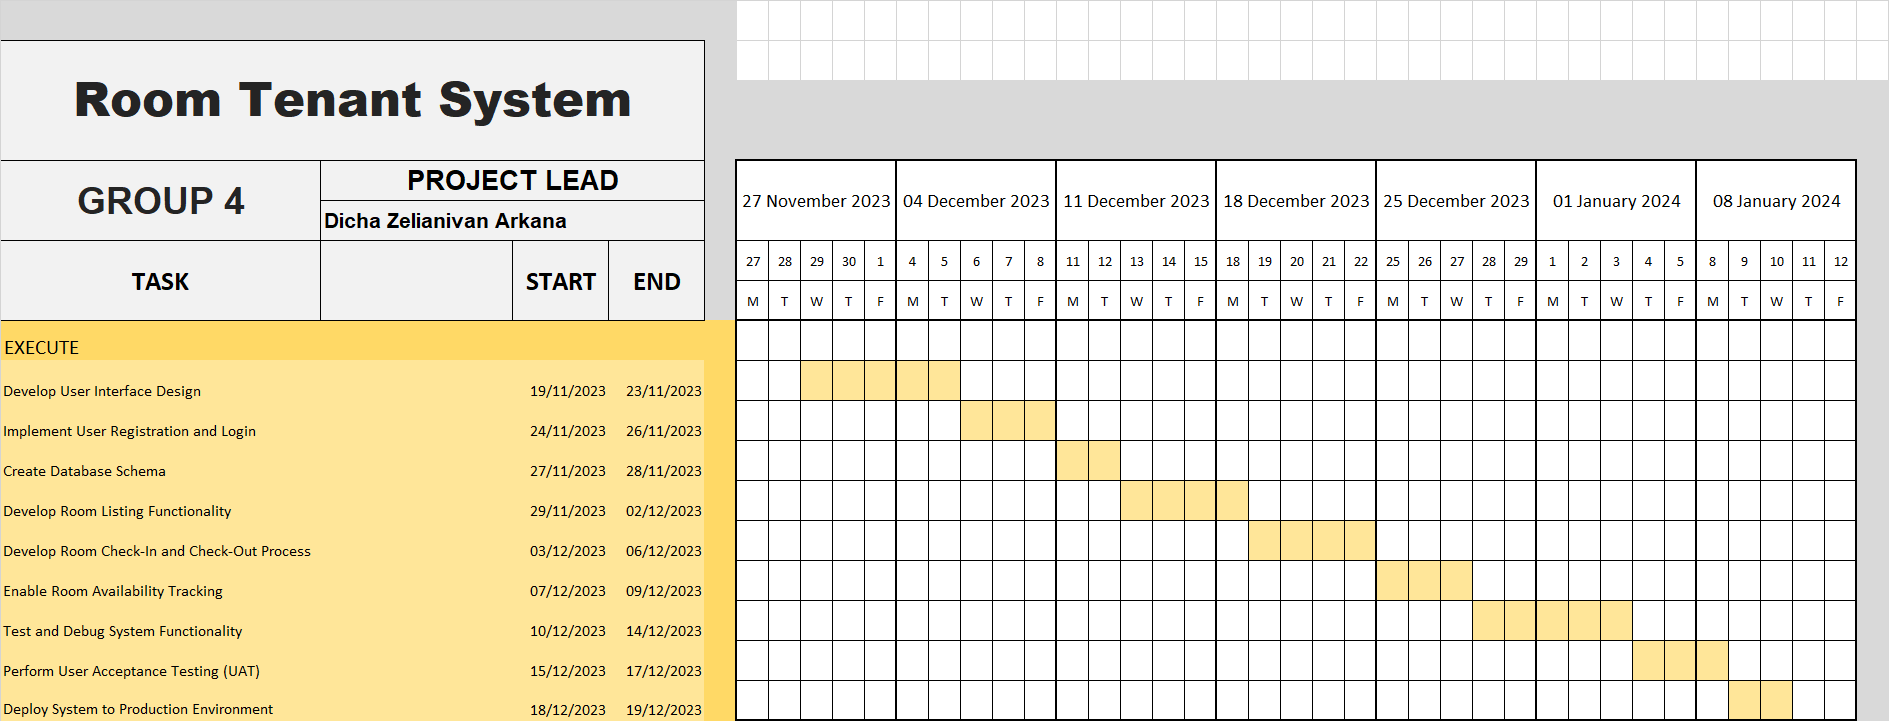
\includegraphics[width=\textheight]{images/figures/gant-Exec.png}
    \end{turn}\\
    \begin{turn}{90}
        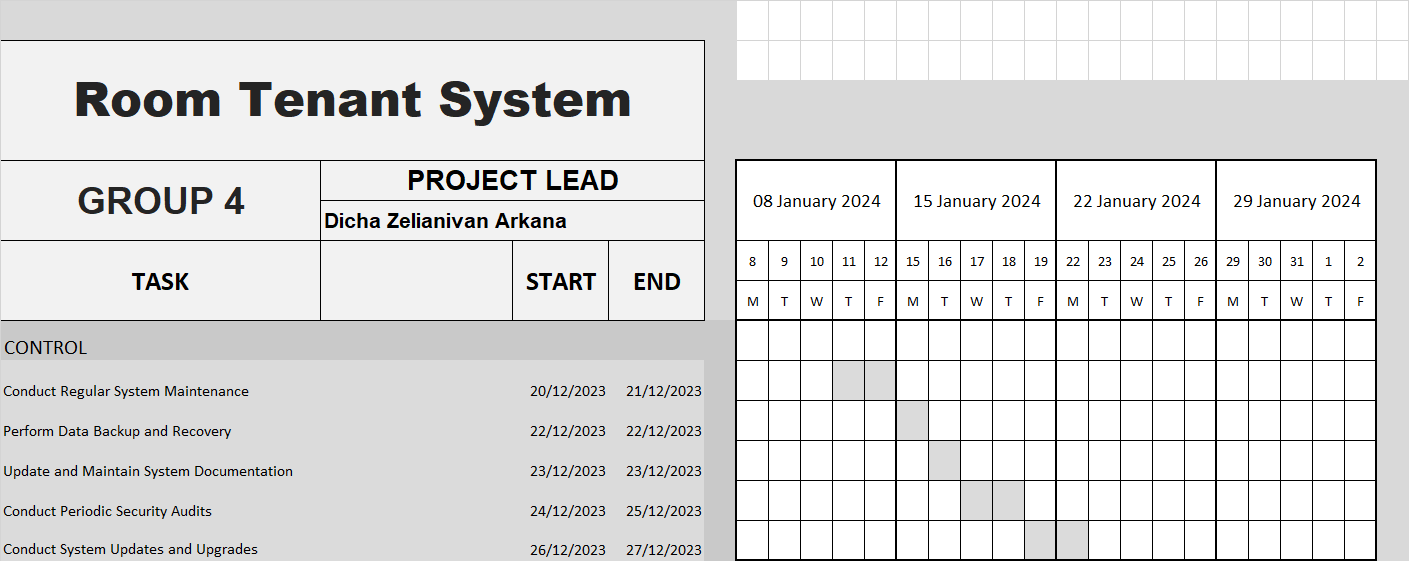
\includegraphics[width=\textheight]{images/figures/gant-Ctrl.png}
    \end{turn}\\
    \begin{turn}{90}
        \includegraphics[width=\textheight]{images/figures/gant-Close.png}
    \end{turn}\\
    \begin{turn}{90}
        \includegraphics[width=\textheight]{images/figures/gant-chart2.png}
    \end{turn}\\
    \section{Technology Stack}
    \resizebox{\textwidth}{!}{
        \begin{tabular}{|p{2.7cm}|p{4.5cm}|p{4.5cm}|}
            \hline
                & \textbf{Languages} & \textbf{Technologies} \\
            \hline
            \textbf{Backend} & PHP, Javascript & IntelliJ Idea \\
            \hline
            \textbf{Frontend} & HTML, CSS & IntelliJ Idea \\
            \hline
            \textbf{Interface} &   & Figma \\
            \hline
            \textbf{Database} & MSSQL &   \\
            \hline
            \textbf{Project Management} &   & Notion, Google Doc, Whatsapp, and Github\\
            \hline
            \textbf{Server} & & Docker \\
            \hline
        \end{tabular}
    }
\chapter{Software Requirement}
    \section{Interface System}
    \begin{center}
        \includegraphics[width=.6\textwidth]{images/figures/Diagram/UI.dio.png}
    \end{center}
    \section{System Design}
    \begin{center}
        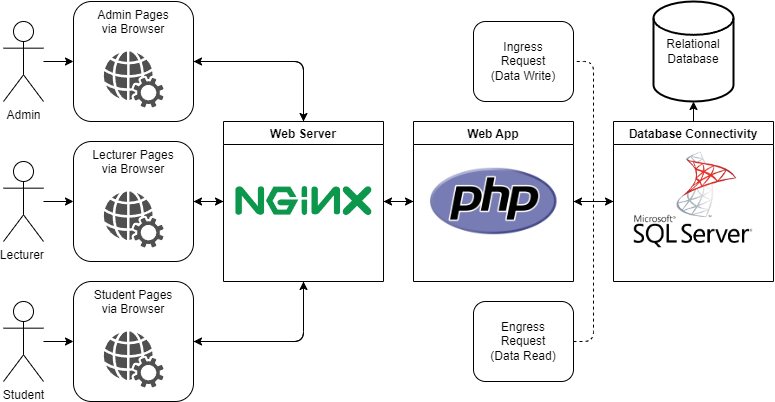
\includegraphics[width=\textwidth]{images/figures/Diagram/SystemDesign.dio.png}
    \end{center}
%     \section{Requirement Gathering}
% \chapter{Software Architecture Document}
%     \section{Use-Case Diagram}
%     \section{Database Schema}
%         \subsection{Tabel Master}
%         \subsection{Tabel View}
\chapter{User Interface and User Experience Document}
    \section{Application Logo}
    \begin{center}
        
\includegraphics[width=6cm]{images/figures/UIUX/logo_jti_baru.png}
    \end{center}
    \section{Application Logo Philosophy}
    The logo is taken from the logo of the information technology major from state polytechnic of malang itself. This logo is used because the app that we created is used for room tenant system to be used in the information technology. So we use the logo of the major itself to make it clear that the app that is being use is used for and belong to the information technology major.
    \newpage
    \section{Color Palet}
    \begin{center}
        \includegraphics[width=2cm]{images/figures/UIUX/Untitled.png}
    \end{center}
    \subsection*{Cyprus (\#0F1E43)}
    The color Cyprus is a tertiary color with hex \#0F1E43. This color is a Combination of primary and secondary colors which typically contain two words. The RGB in a color space for this color has three components: 15\%, 30\%, and 67 . Additionally, this cool color has HSB color space, which consists of \% 223, \% 77.61, and \% 26.27. pbl
    \begin{center}
        
\includegraphics[width=2cm]{images/figures/UIUX/Untitled 1.png}
    \end{center}
    \subsection*{Thunderbird (\#984934)}
    Color Thunderbird is from the neutral family. Therefore, it is very useful and has a good coexistence with other colors. Its RGB color space consists of\% 152\%, 57\%, and 52. The numbers undefined, undefined and undefined also indicate the different values of the LAB color space of this color, respectively. Finally, its HSL color space consists of\% h3, \% 49, and \% 40.
    \begin{center}
        
\includegraphics[width=2cm]{images/figures/UIUX/Untitled 2.png}
    \end{center}
    \subsection*{Cinnabar (\#F15528)}
    Cinnabar color with hex code \#F15528 is probably the most widely used color among users. Its constituent hue is also a secondary color. Its HSB color space is\% 13,\% 83.4 and\% 94.51. The values R22, 16 and 94.51 also make up its NCol color code.
    \begin{center}
        \includegraphics[width=2cm]{images/figures/UIUX/Untitled 3.png}
    \end{center}
    \subsection*{Dark Tangerine (\#F99C1D)}
    Hue that makes up Dark Tangerine is one of the primary colors. Many designers like this color with the hex code \#F99C1D. CMYK color space with values of\% 0, \% 88, \% 88, and \% 2 constitute this color. Its Pantone color code values are also 15-1058 TCX.
    \begin{center}
        \includegraphics[width=2cm]{images/figures/UIUX/Untitled 4.png}
    \end{center}
    \subsection*{Amber (\#FEBE10)}
    The color Amber is a tertiary color with hex \#FEBE10. This color is a Combination of primary and secondary colors which typically contain two words. The RGB in a color space for this color has three components: 254\%, 190\%, and 16 . Additionally, this cool color has HSB color space, which consists of \% 44, \% 93.7, and \% 99.61.
    \section{User Flow}
    \subsection{General Description}
    The Room Tenant System is designed to optimize the room rental experience by involving three main roles: User, Admin, and Approver. The main goal of this system is to ensure the rental process is easier by digitalization, transparency, and in accordance with applicable requirements and policies.
    \subsection{Users and Personas}
    \begin{enumerate}[label=\alph*.]
        \item User
        Personas
        \begin{itemize}
            \item System users who want to rent space for certain purposes.
            \item Diverse users from various backgrounds and needs.
        \end{itemize}
        \item Admin
        Personas
        \begin{itemize}
            \item System administrator responsible for general management and monitoring rental activities.
            \item Have access to full control of system data and settings.
        \end{itemize}
        \item Approver
        Personas
        \begin{itemize}
            \item The party who has the authority to approve or reject room rental requests.
            \item Ensure compliance with established policies and requirements.
        \end{itemize}
    \end{enumerate}
    \subsection{User flow for user}
    \noindent
    \includegraphics[width=\textwidth]{images/figures/UIUX/Untitled 5.png}
    General Steps :
    \begin{enumerate}
        \item Users access the room tenant system website
        \item To access website services, users need to log in first with the account they already have.
        \item The user already logged in to the system.
        \item At this point (home), the user can see the rooms available to borrow and three available menus.
        \item Users can directly select an available room at home or go to the room list menu to select the room they want to borrow.
        \item When the user has determined the room he wants to borrow, the user needs to fill in a borrow detail form consisting of the name of the event, date and time, as well as event details.
        \item Apart from filling in borrow details, users need to agree to the code of conduct of the relevant regulations and room.
        \item After everything has been filled in correctly by the user, the user can click the submit button to submit a request.
        \item The user has finished making a borrow request.
    \end{enumerate}
    Validation and Error Handling :
    \begin{enumerate}
        \item It happens on the login process, If the account credentials entered are correct then the user can log in and arrive at the home page. But when the credentials 5entered are incorrect, the user is asked to log in again and ensure that the credentials entered are correct.
        \item When a user has submitted a borrow request, when the system finds a borrow request on the same date and time in the room desired by the user, the system will ask the user to change the date and time that does not collide.
    \end{enumerate}
    Backtracking :\\
    Users can only abandon their intention to borrow the room they choose only when they have not submitted it. At the point where the user is asked to fill out a borrowed form, he can again use the back button to cancel the room selection.
    \subsection{User flow for admin}
    \noindent
    \includegraphics[width=\textwidth]{images/figures/UIUX/Untitled 6.png}
    General Steps :
    \begin{enumerate}
        \item Admin access the room tenant system website
        \item Admin login using their username and password.
        \item After logging in, the admin will be directed to the homepage where they can view the pending approvals and the statistics of rooms.
        \item Admin can choose pending approval on the homepage then fill in the approver detail, this is needed to forward borrow request to the related approver
        \item The admin can also access the "Room List" menu, where they can create, edit, and delete rooms using the provided buttons.
        \item To add a new room, the admin can click on the "Add New Room" button and fill in the room details, including the room name, code, floor, side, capacity, and cover image.
        \item If the admin wants to edit the details of an existing room, they can select the room from the room list and click on the "Edit" button.
        \item To delete an existing room, admin can select the room from the room list and click on the “Delete” button.
        \item Admin can access the "User List" page to view the list of system users.
        \item Admin can add a new user by clicking the "Create New User" button and filling in user details such as name, class and student ID.
        \item If the admin wants to edit the details of an existing user, they can select the user from the user list and click the "Edit" button.
        \item Admin can also delete a user by selecting the user from the user list and clicking the "Delete" button.
        \item The admin can also view the upcoming events on the "Event List" page.
    \end{enumerate}
    Validation and Error Handling :\\
    During the login process, if the entered account credentials are correct, the adm\\in can log in and access the homepage. If the credentials are incorrect, the admin will be prompted to log in again and ensure the credentials are correct.\\
    Backtracking :\\\\
    The admin can navigate back to the previous page using the back button on each menu.
    \newpage
    \subsection{User flow for approver}
    \noindent
    \includegraphics[width=\textwidth]{images/figures/UIUX/Untitled 7.png}
    General Steps :
    \begin{enumerate}
        \item The approver logs in using their username and password.
        \item After logging in, the approver is directed to the homepage where they can view the list of pending approvals.
        \item If the approver selects a specific approval from the list, they will be directed to the approval details page where they can approve or reject the request.
        \item The approver can also view the history approved request on the "Approved" page.
    \end{enumerate}
    Validation and Error Handling :\\
    During the login process, if the entered account credentials are correct, the approver can log in and access the homepage. If the credentials are incorrect, the approver will be prompted to log in again and ensure the credentials are correct.\\\\
    Backtracking :\\
    The approver can navigate back to the previous page using the back button on each menu.
    \newpage
    \section{Wireframe (Low-fidelity Design)}
    \subsection{User}
    \begin{center}
        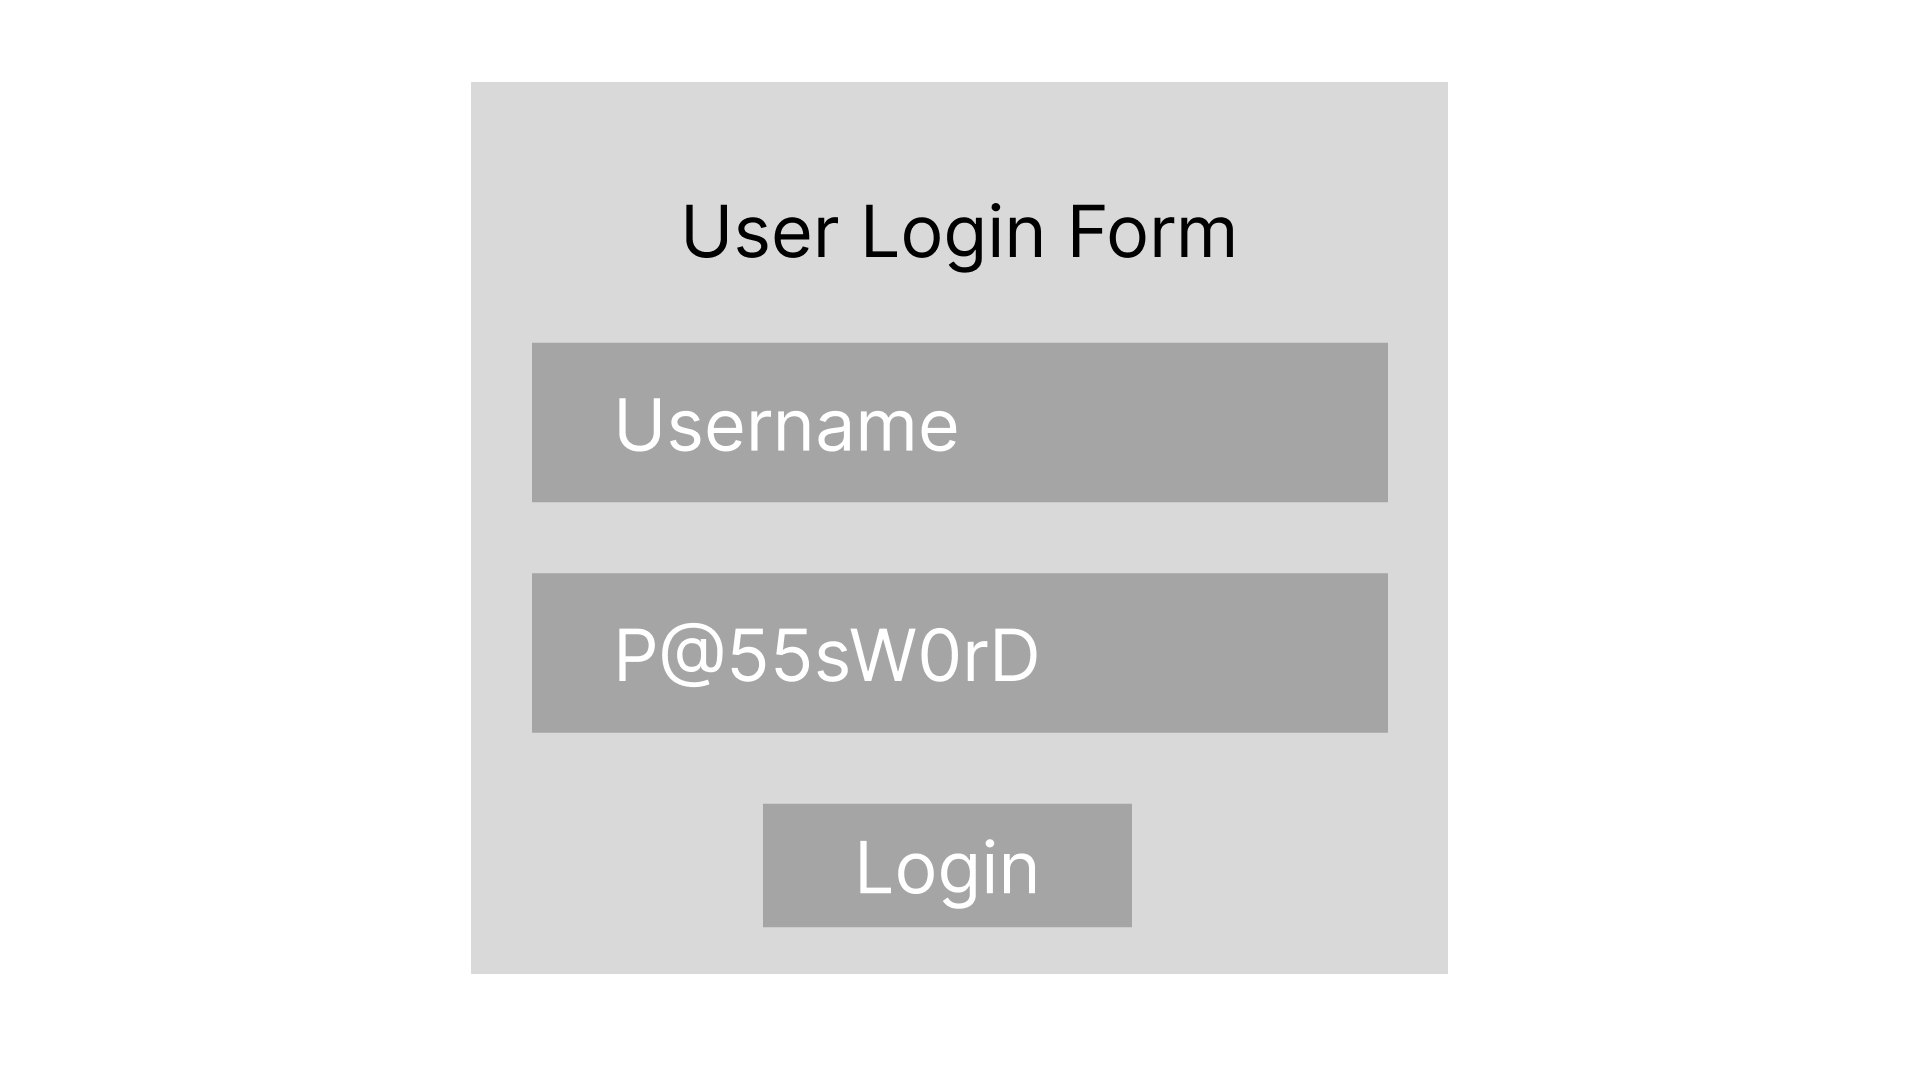
\includegraphics[width=\textwidth]{images/figures/UIUX/Login_Page_(Atmin).png}\\
        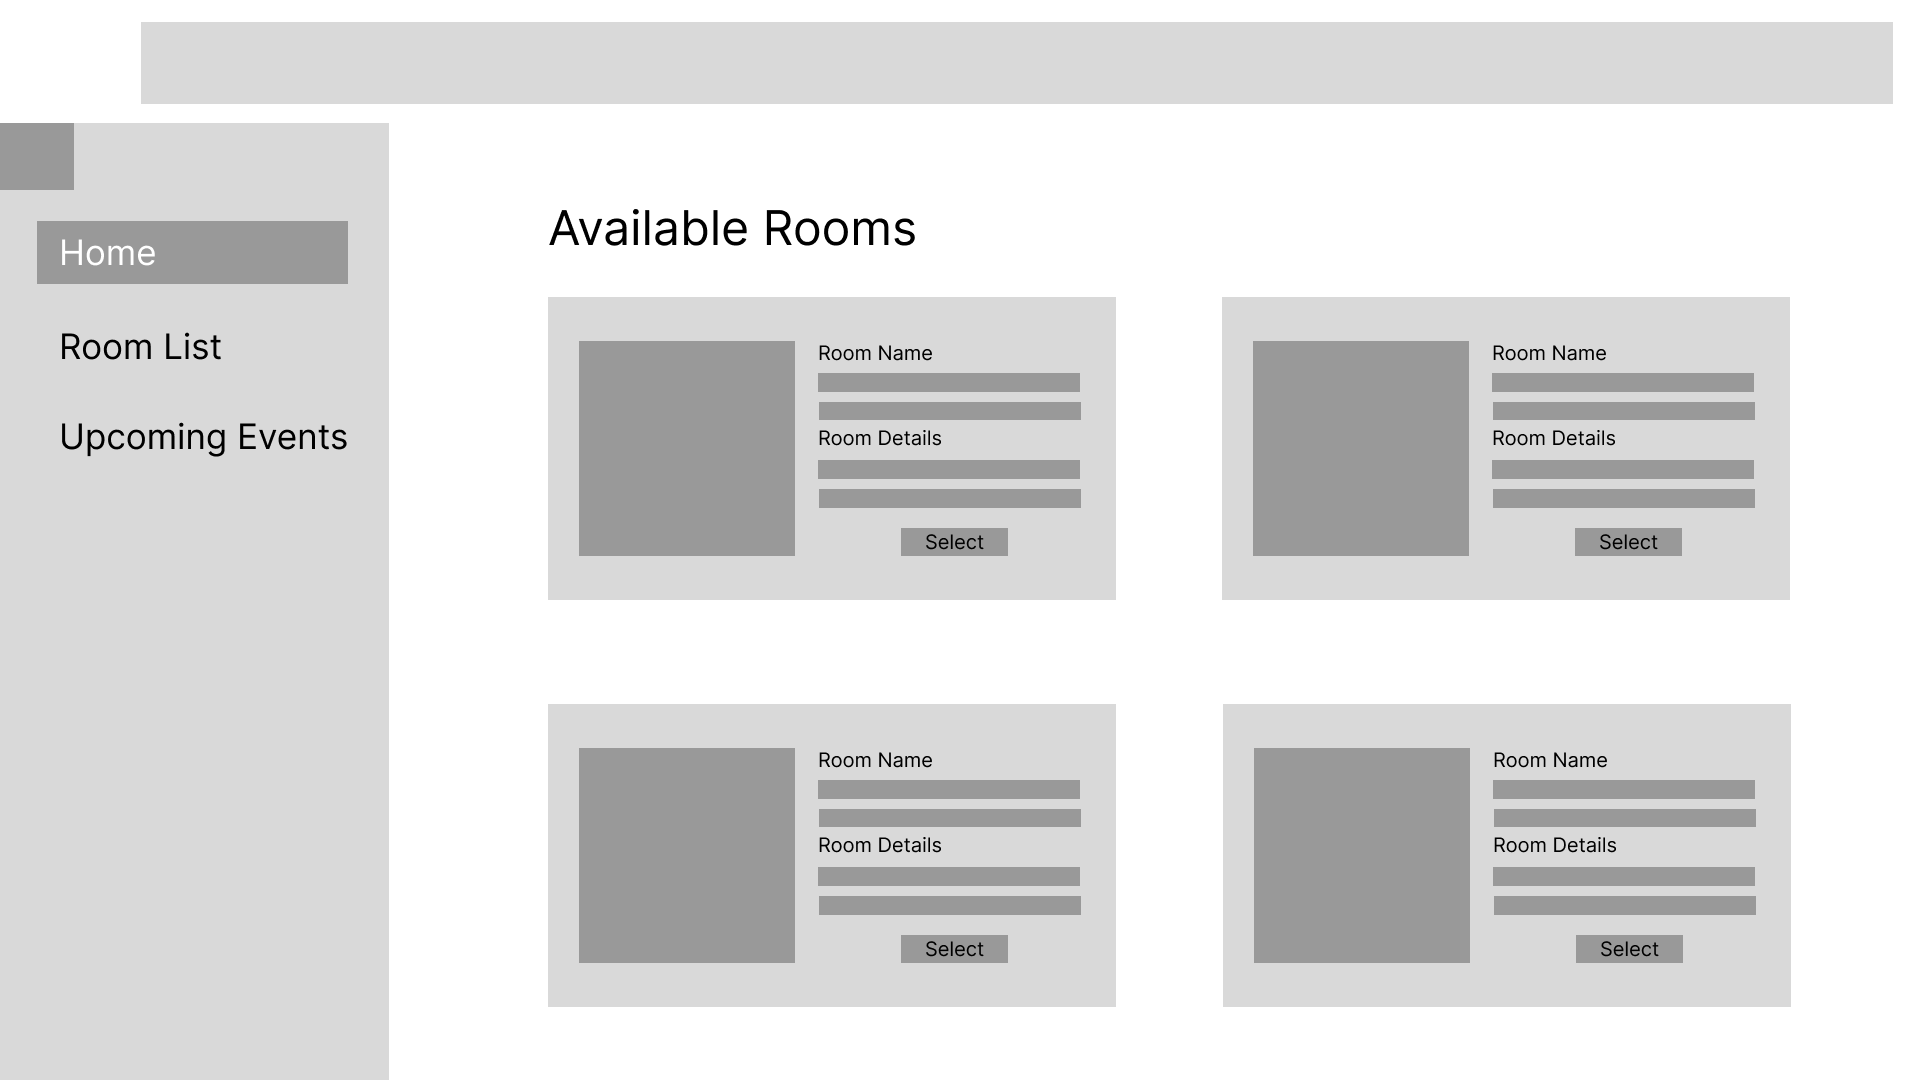
\includegraphics[width=\textwidth]{images/figures/UIUX/Room_Borrowing_Page_(User).png}\\
        \includegraphics[width=\textwidth]{images/figures/UIUX/Room_Description_(User).png}\\
        \includegraphics[width=\textwidth]{images/figures/UIUX/Borrowing_Details_Page_(User).png}\\
        \includegraphics[width=\textwidth]{images/figures/UIUX/Room_List_Page_(User).png}\\
        \includegraphics[width=\textwidth]{images/figures/UIUX/Event_List_Page_(User).png}\\
    \end{center}
    \subsection{Admin}
    \begin{center}
        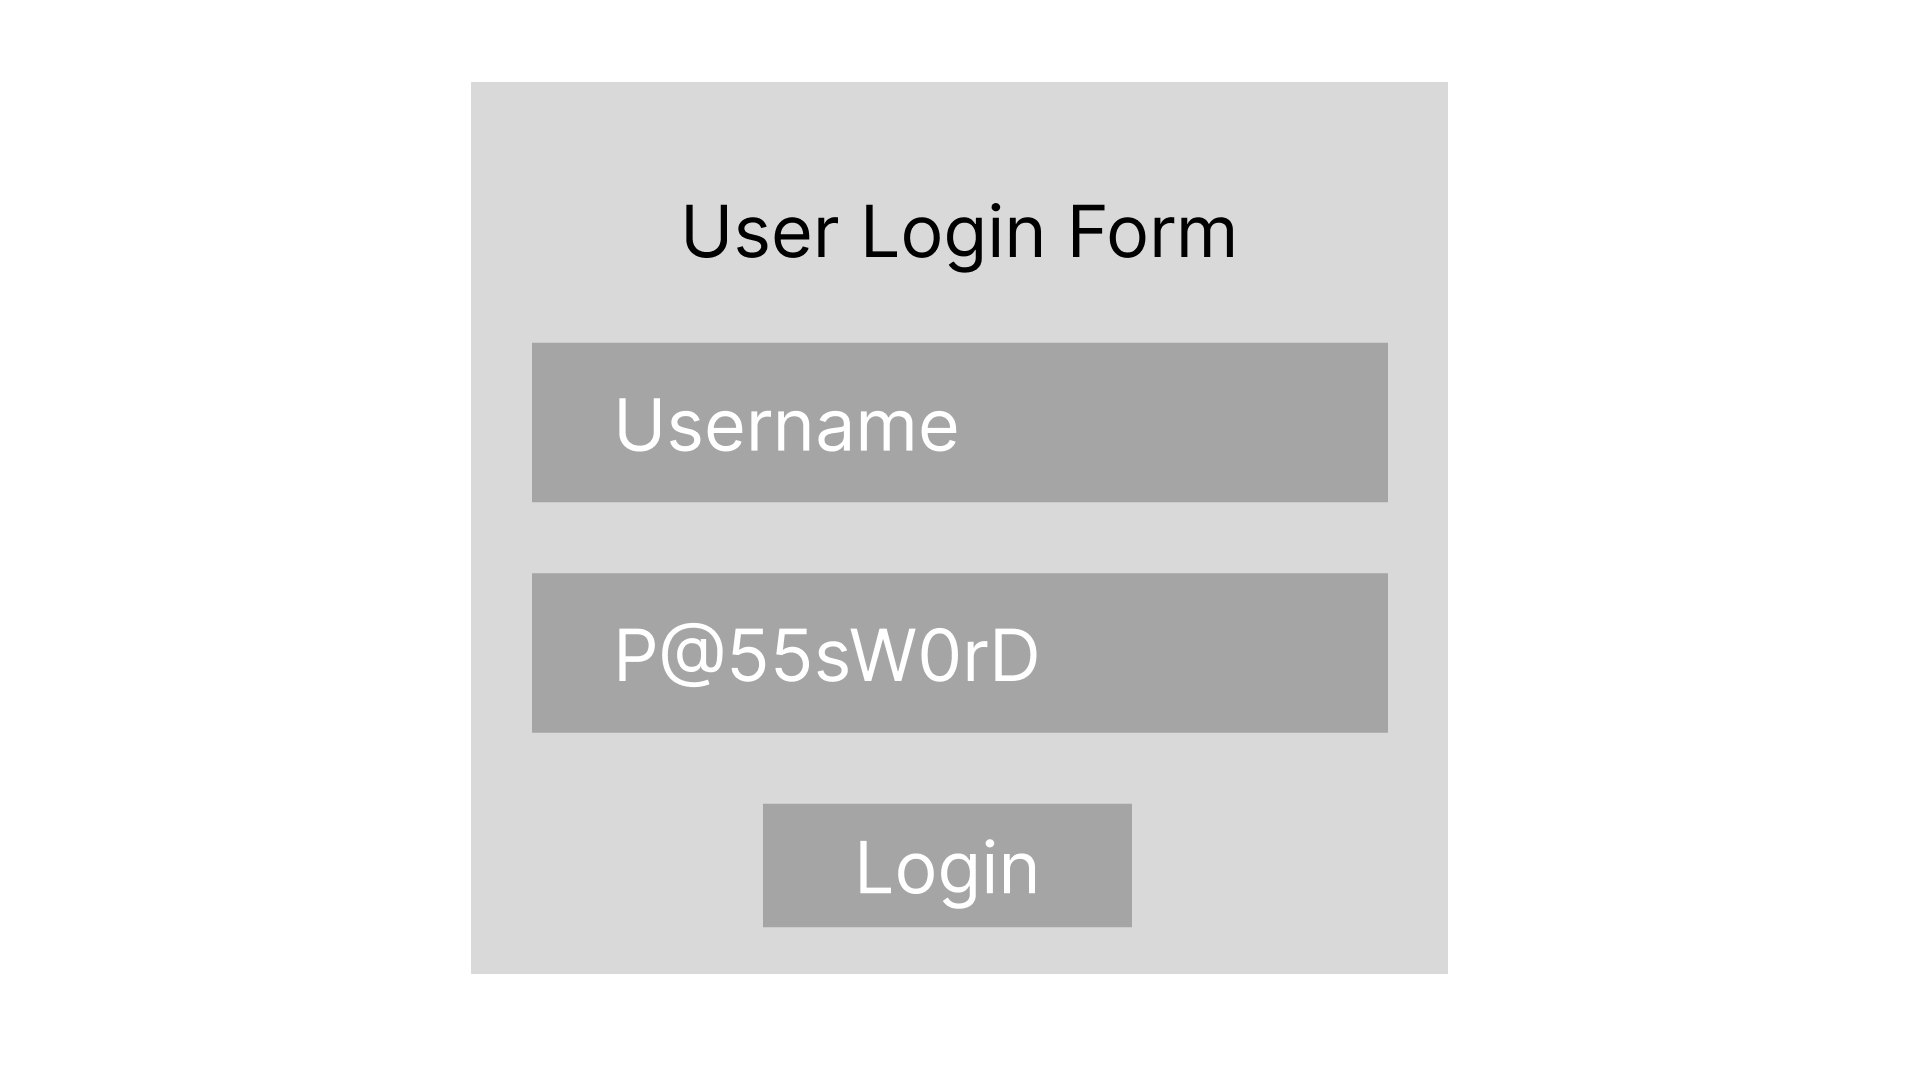
\includegraphics[width=\textwidth]{images/figures/UIUX/Login_Page_(Atmin).png}\\
        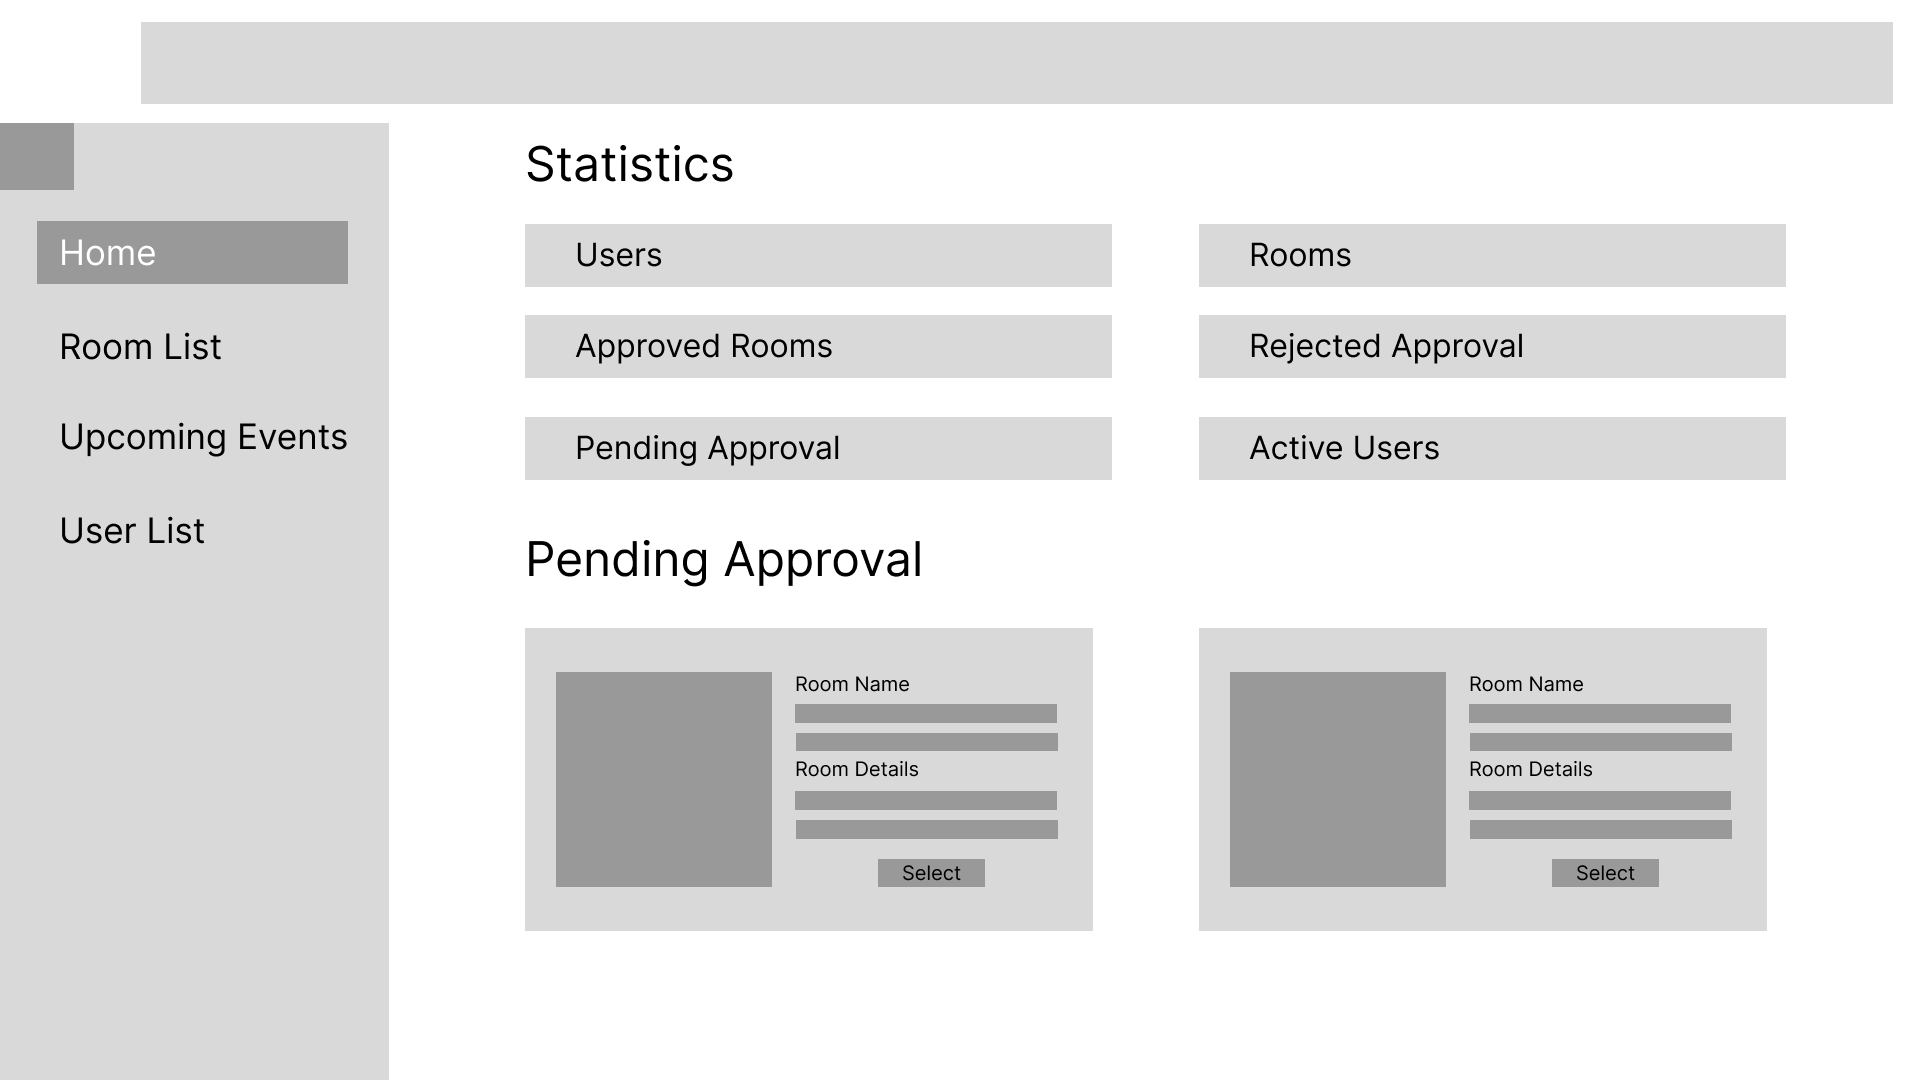
\includegraphics[width=\textwidth]{images/figures/UIUX/Homies_Page_(Atmin).png}\\
        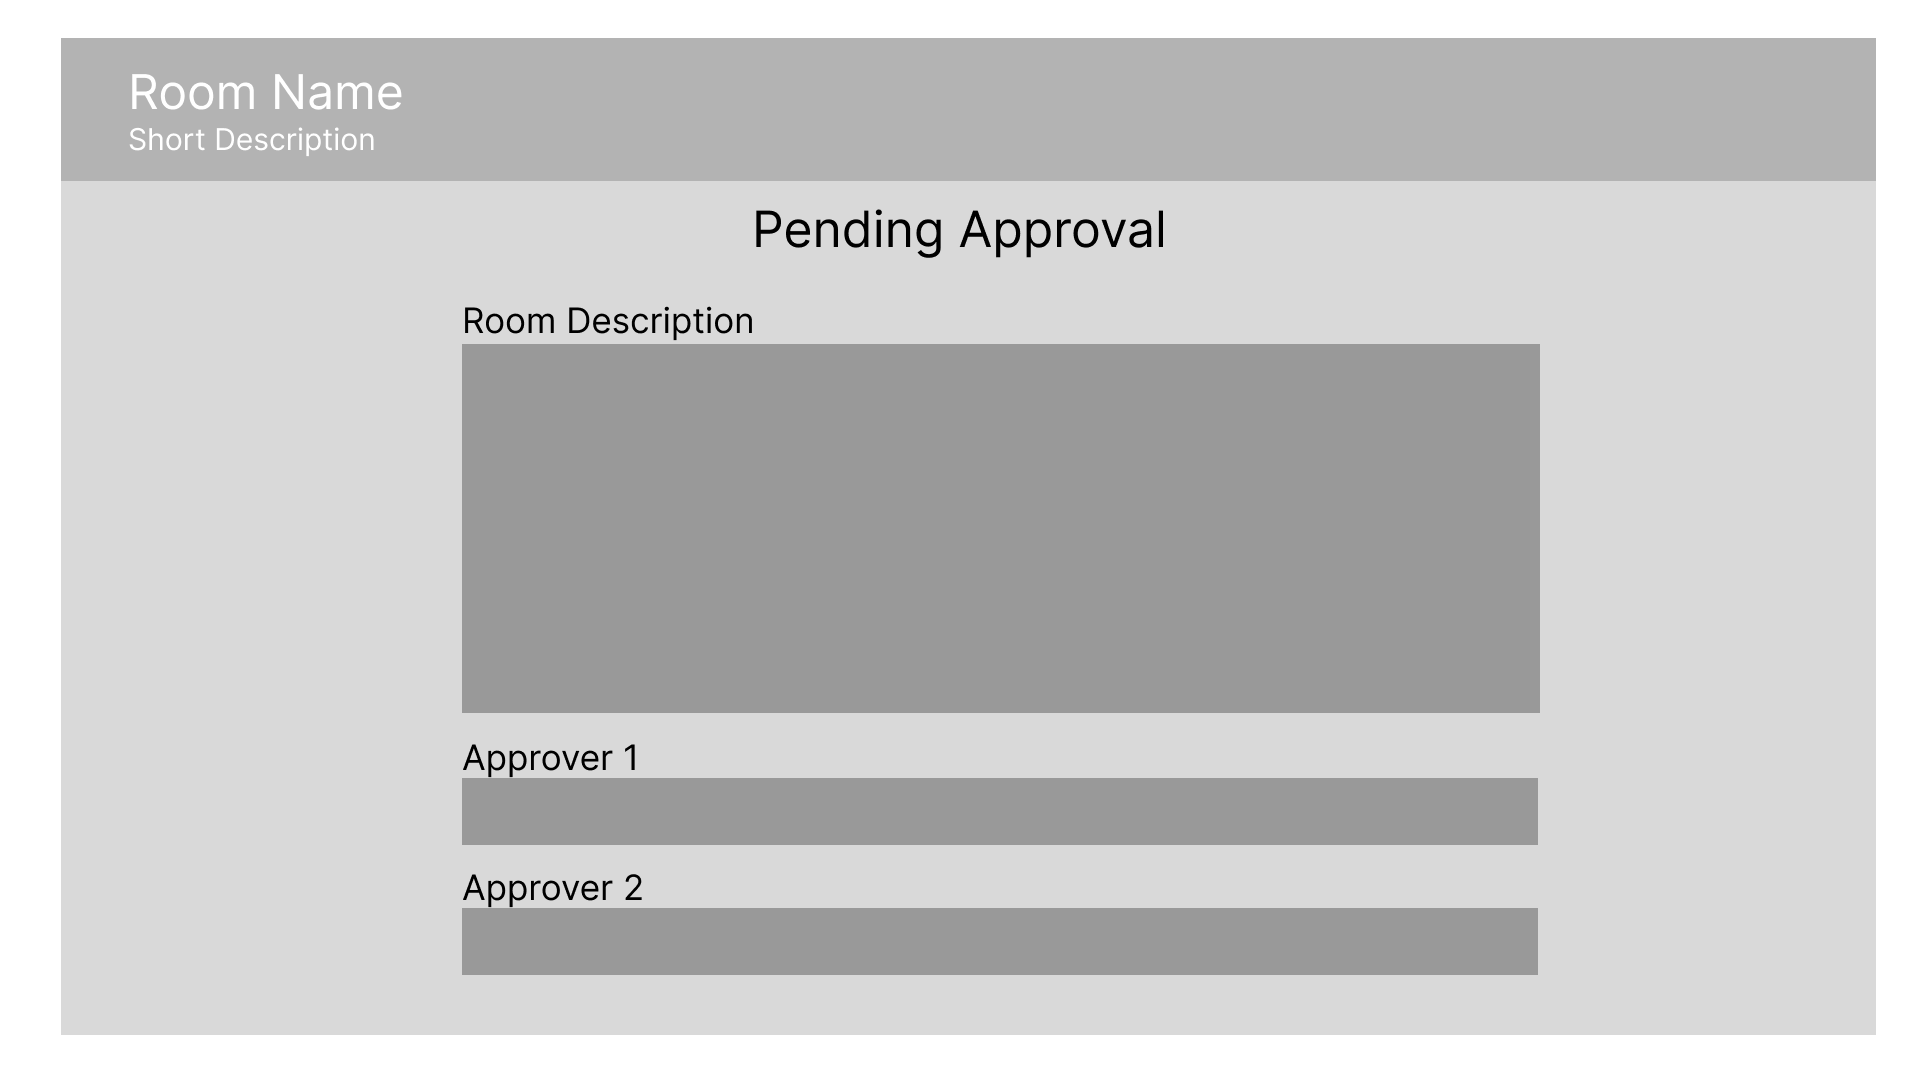
\includegraphics[width=\textwidth]{images/figures/UIUX/Pending_Approval_(Atmin).png}\\
        \includegraphics[width=\textwidth]{images/figures/UIUX/Event_List_Page_(Atmin).png}\\
        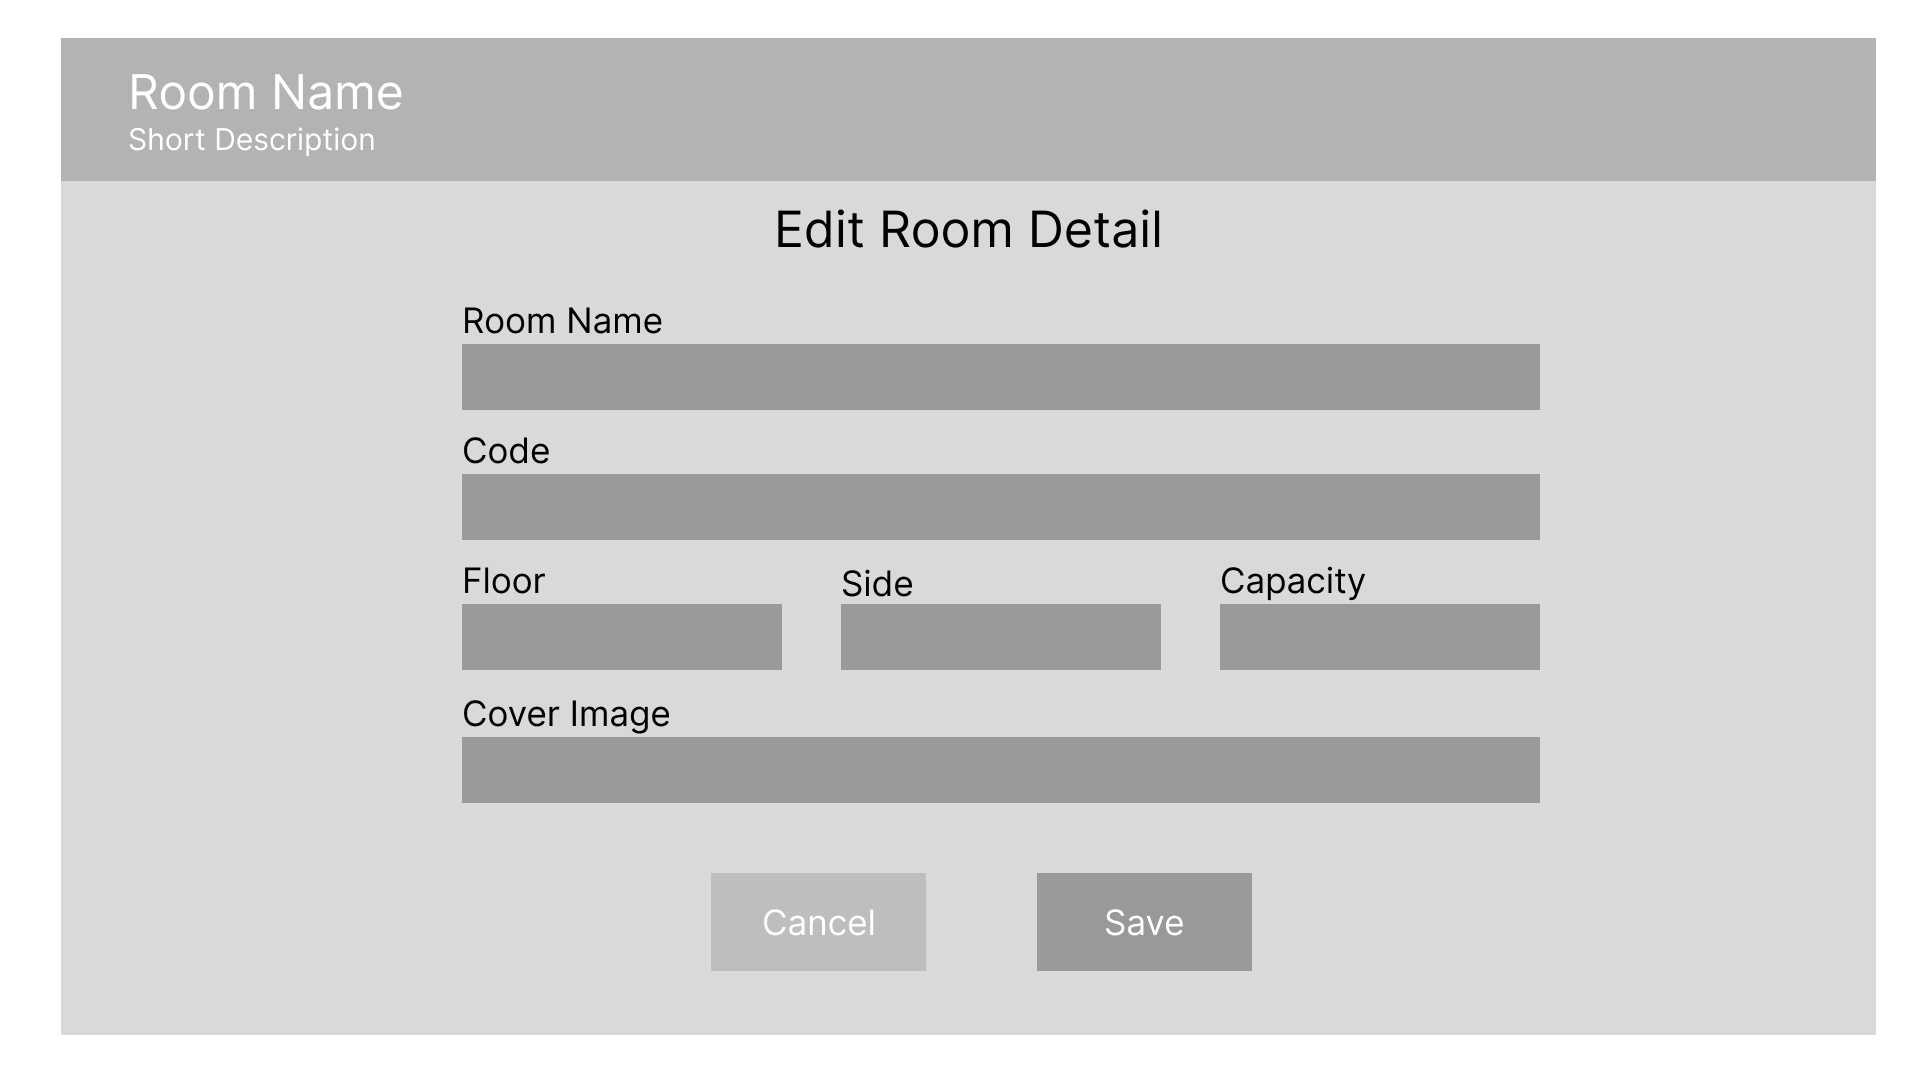
\includegraphics[width=\textwidth]{images/figures/UIUX/Edit_Room_(Atmin).png}\\
        \includegraphics[width=\textwidth]{images/figures/UIUX/Event_List_Page_(Atmin).png}\\
        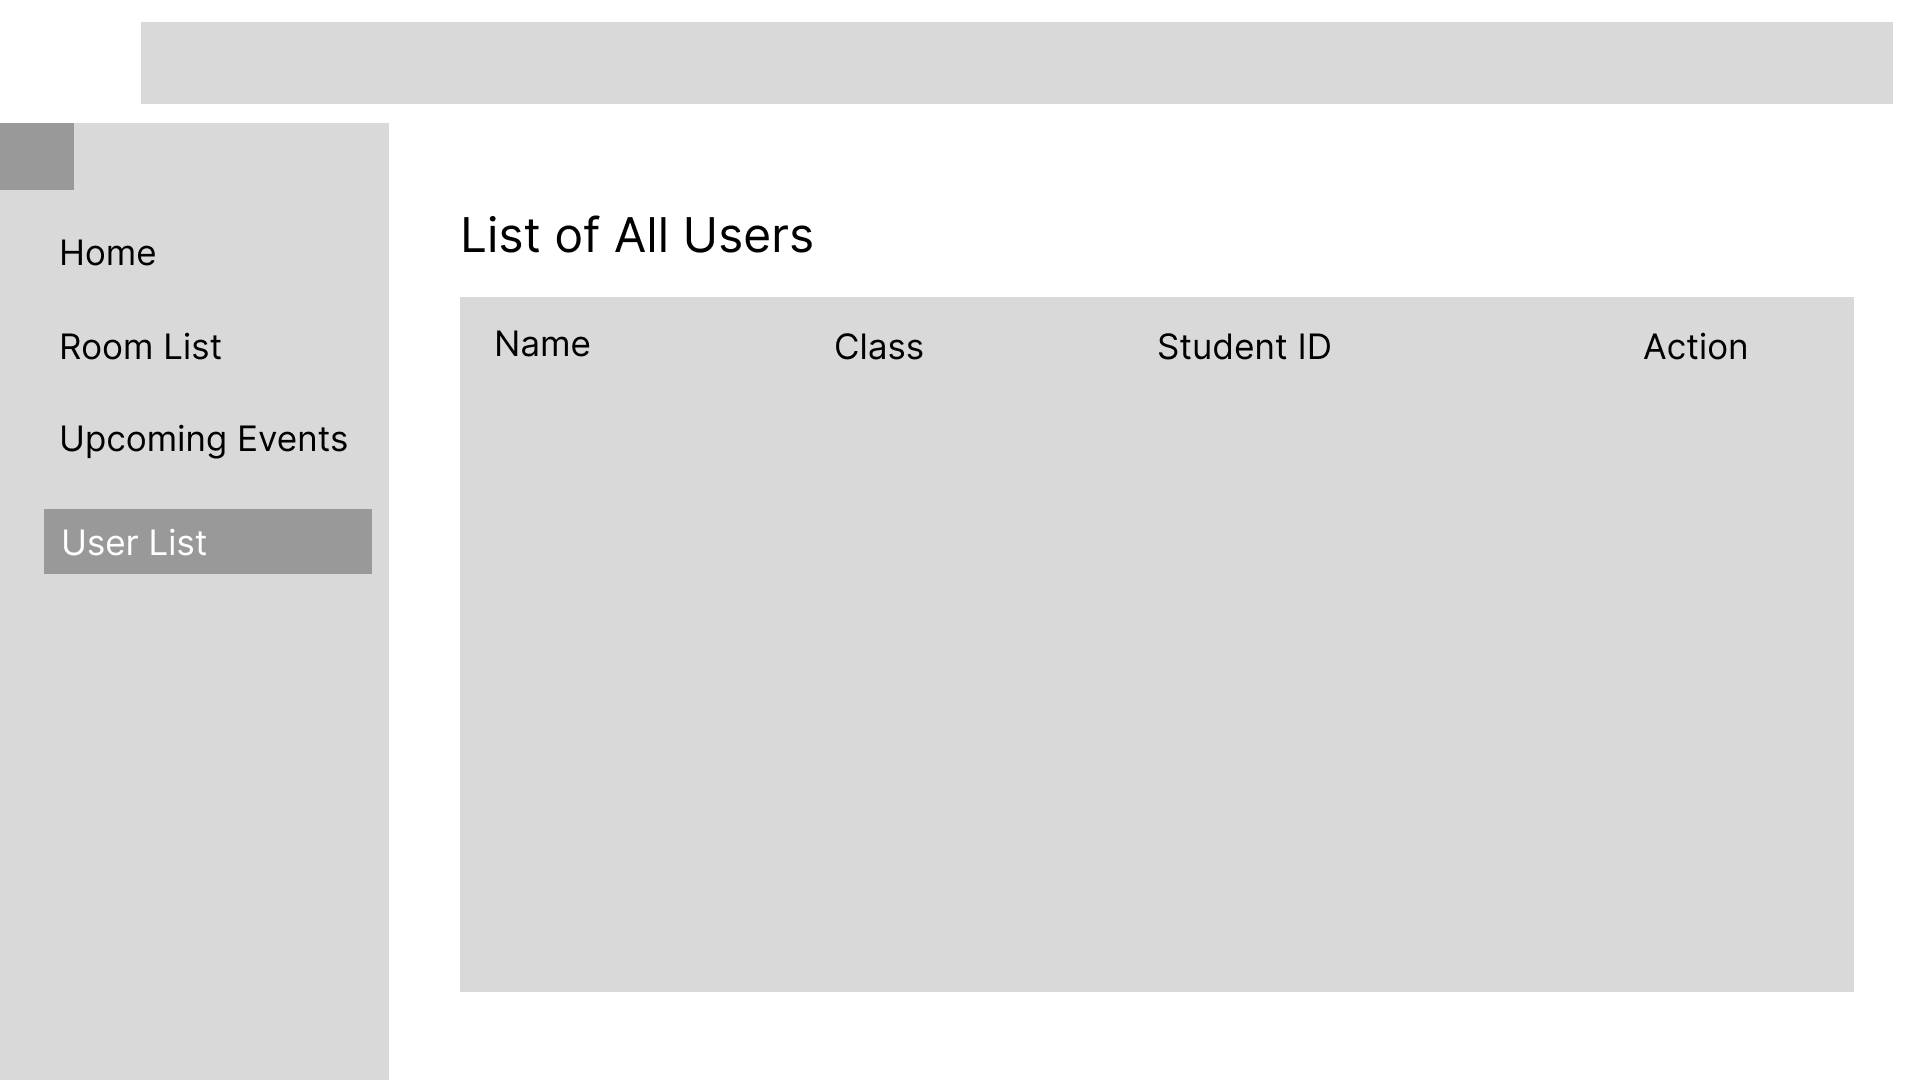
\includegraphics[width=\textwidth]{images/figures/UIUX/User_List_(Atmin).png}\\
        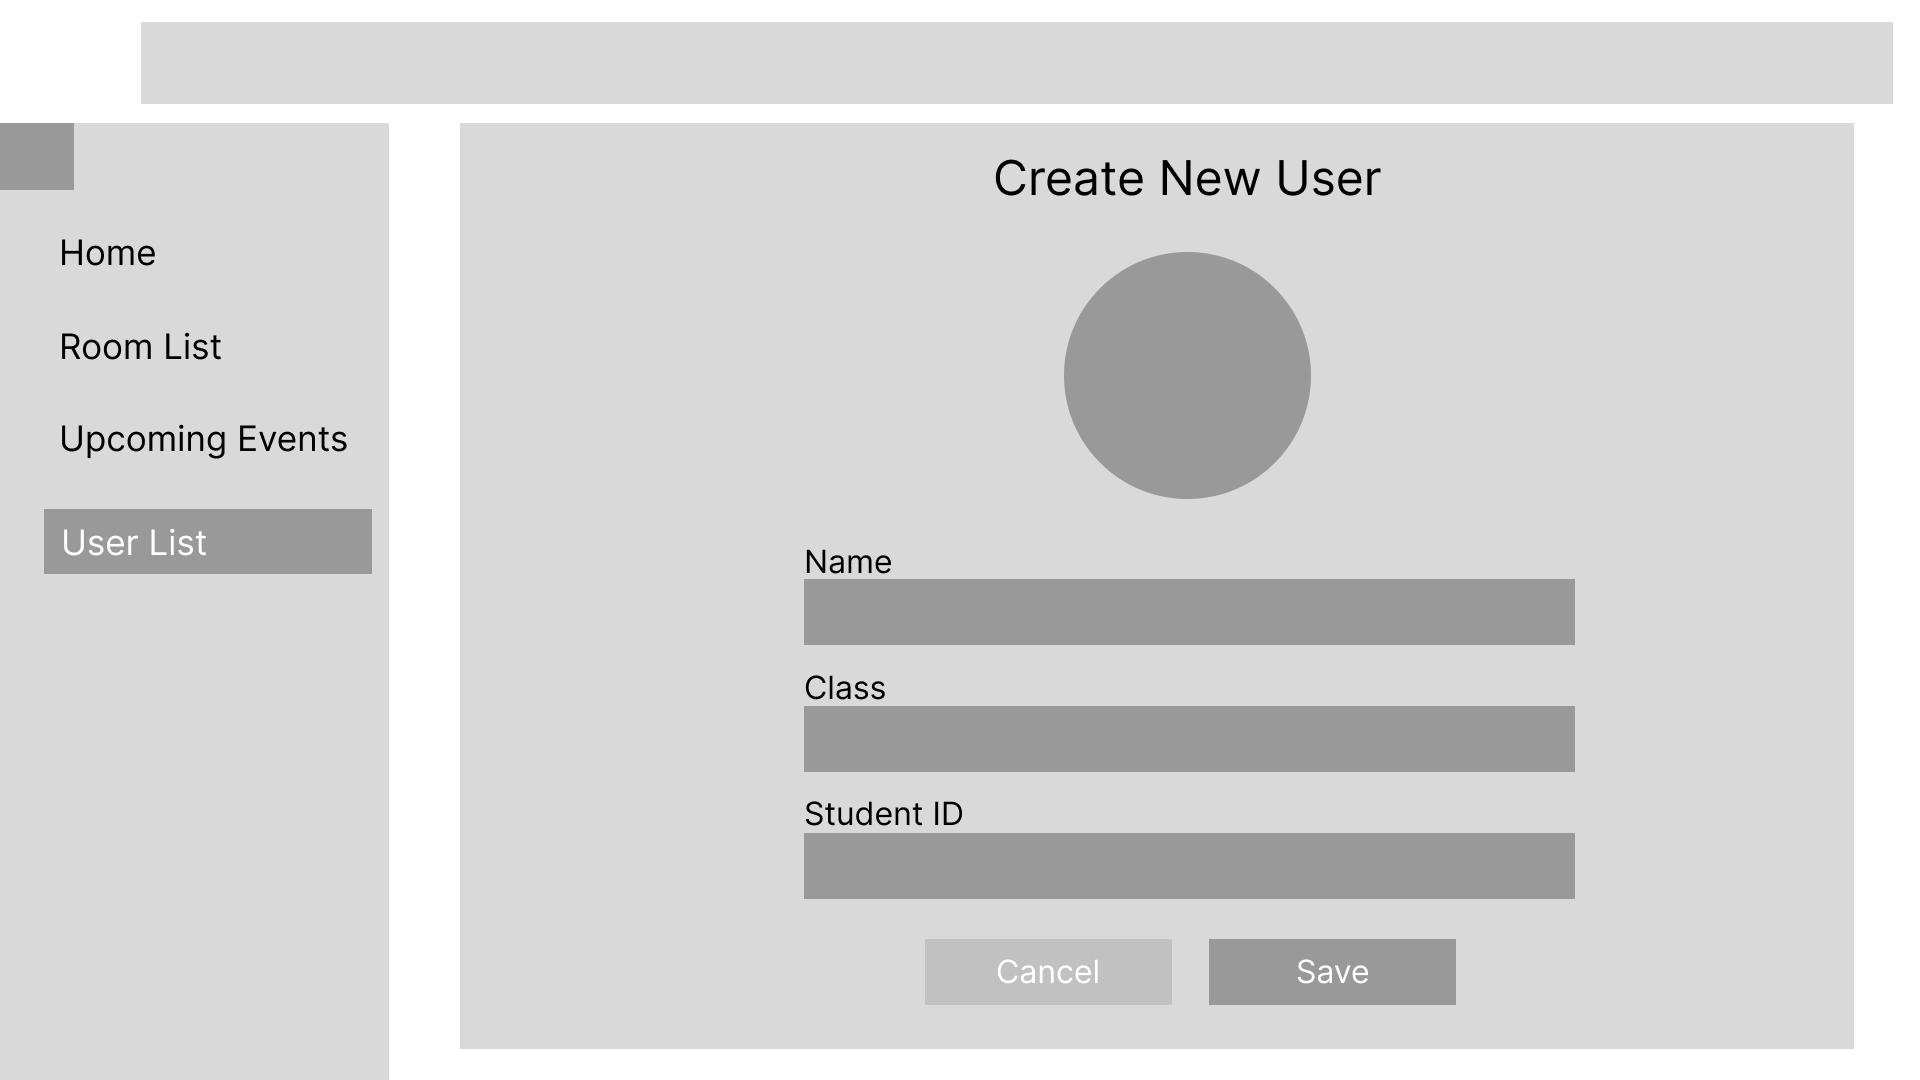
\includegraphics[width=\textwidth]{images/figures/UIUX/Create_New_User_(Atmin).png}\\
        \includegraphics[width=\textwidth]{images/figures/UIUX/Edit_User_(Atmin).png}\\
    \end{center}
    \newpage
    \subsection{Approver}
    \begin{center}
        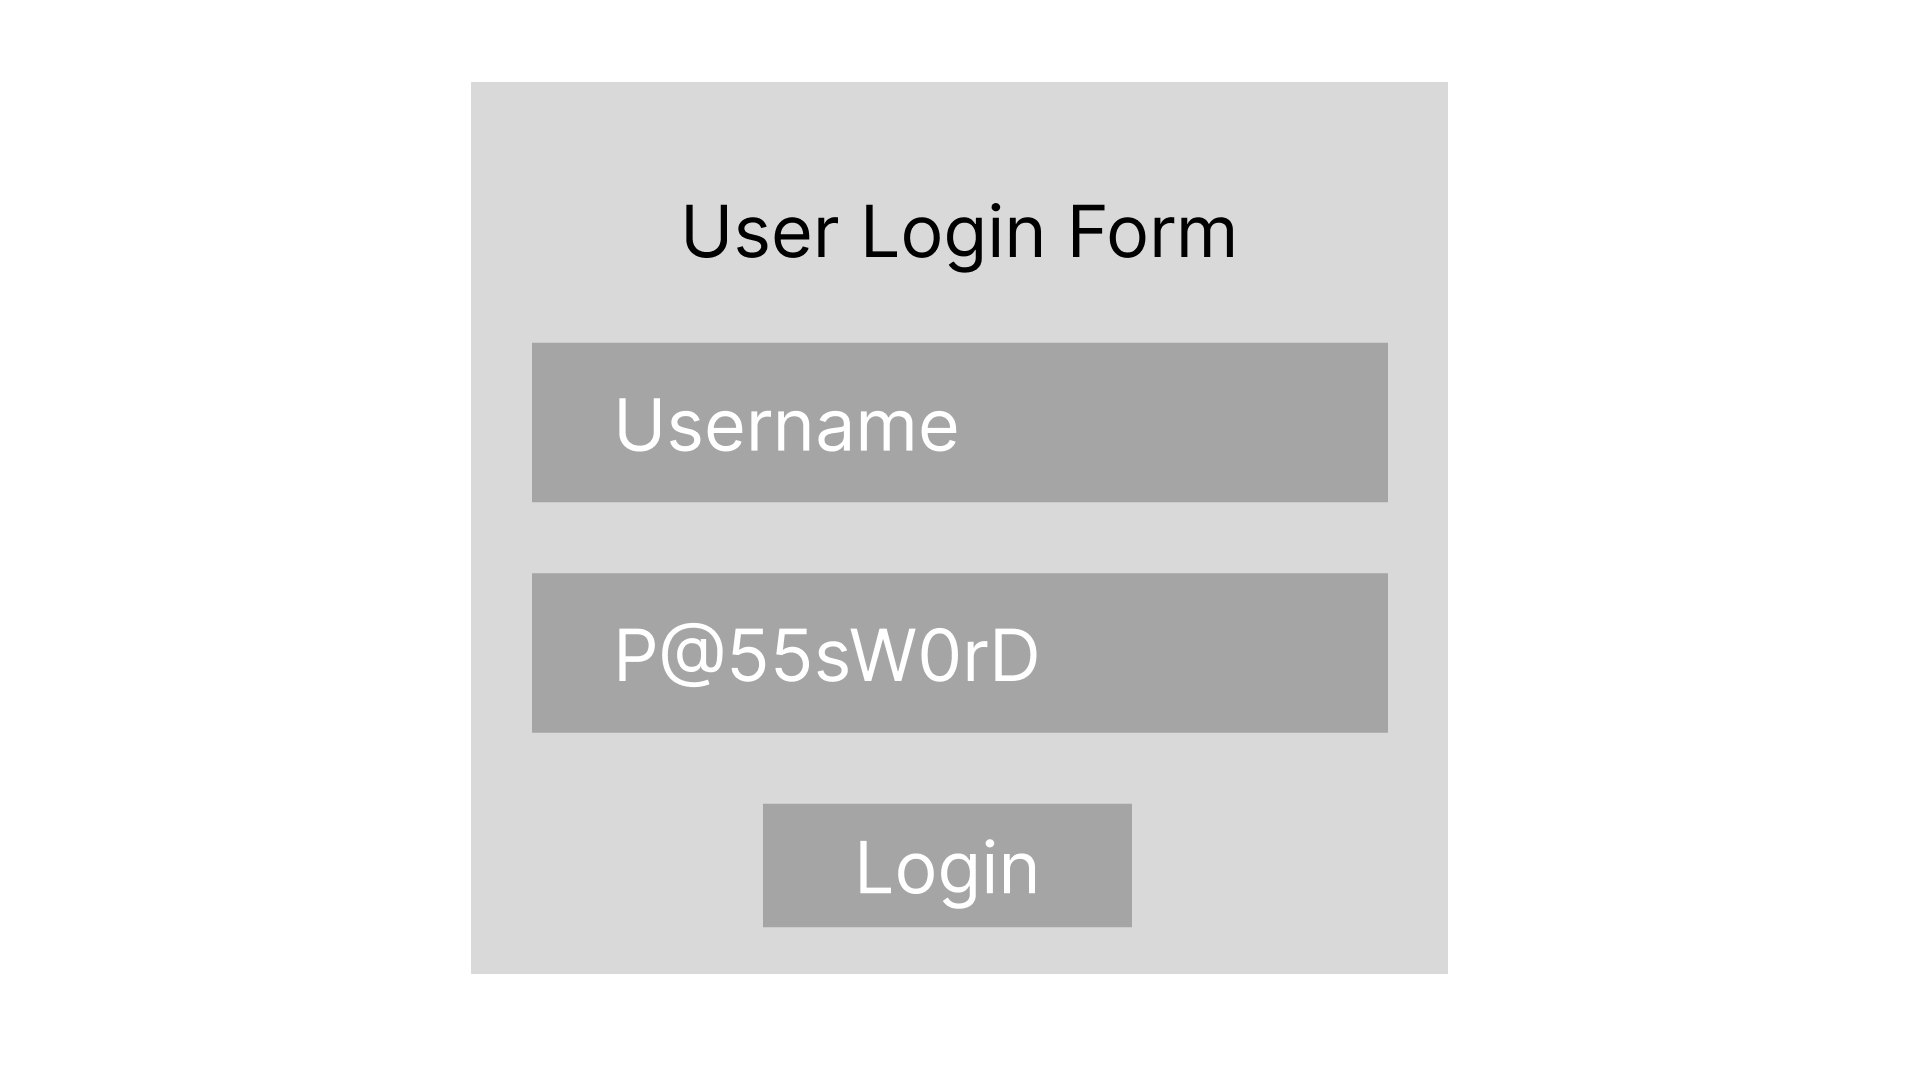
\includegraphics[width=\textwidth]{images/figures/UIUX/Login_Page_(Atmin).png}\\
        \includegraphics[width=\textwidth]{images/figures/UIUX/Room_Borrowing_Page_(Dosenk).png}\\
        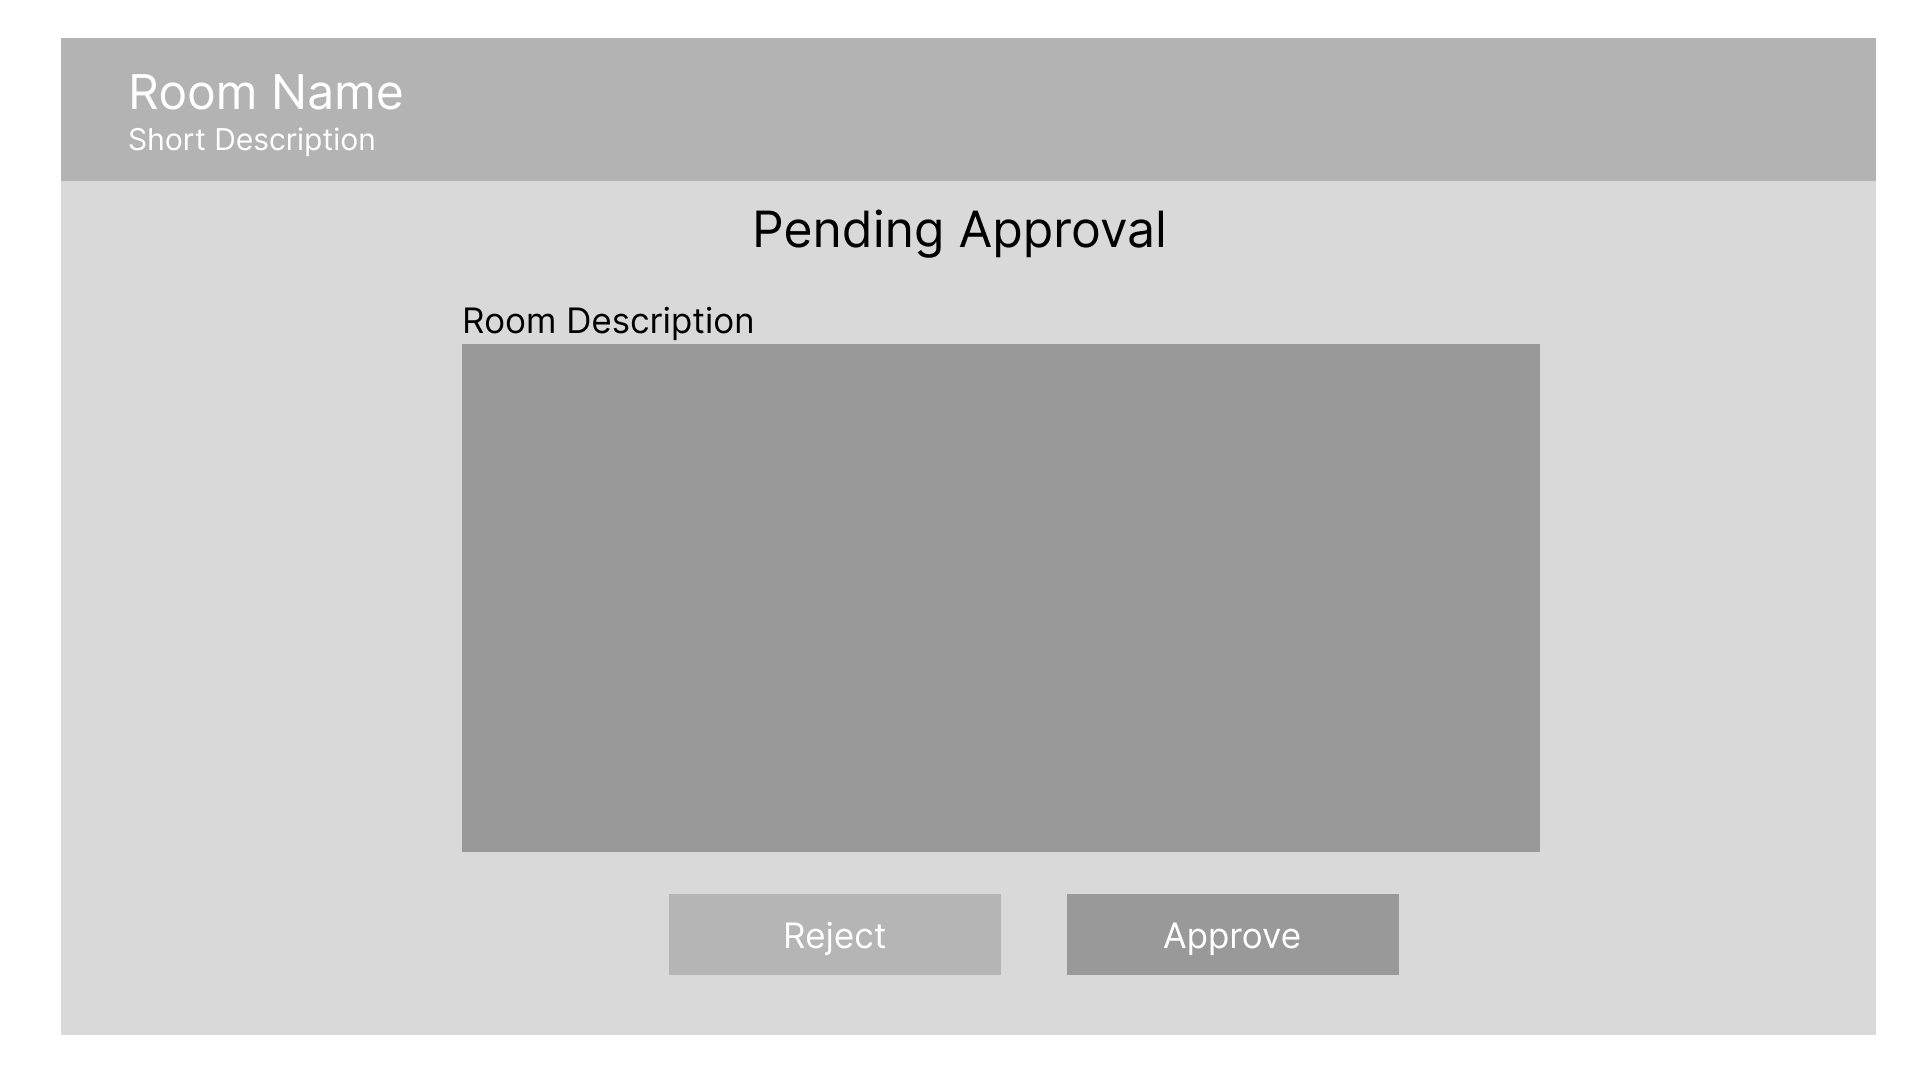
\includegraphics[width=\textwidth]{images/figures/UIUX/Pending_Approval_(Dosenk) 1.png}\\
        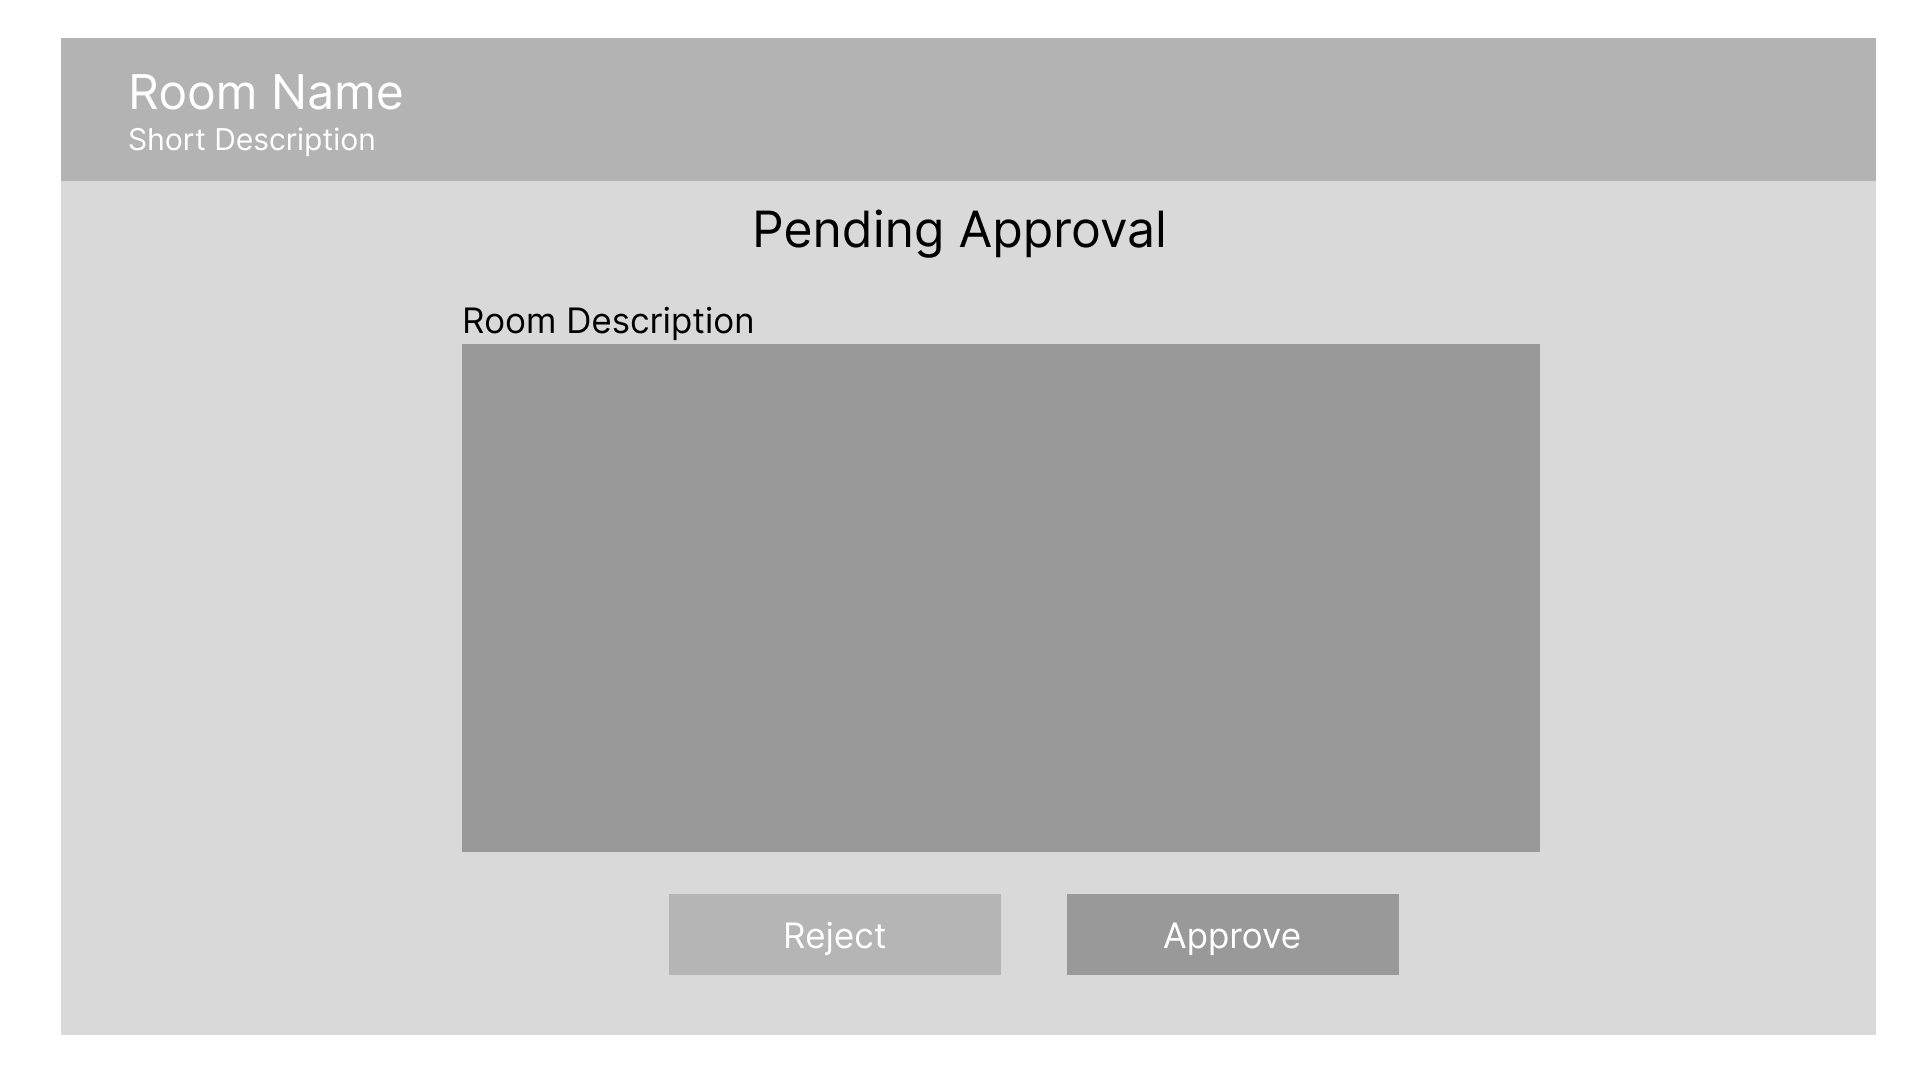
\includegraphics[width=\textwidth]{images/figures/UIUX/Pending_Approval_(Dosenk) 1.png}\\
    \end{center}
    \newpage
    \section{User Interface (High-fidelity Design)}
    \subsection{User}
    \begin{center}
        \includegraphics[width=\textwidth]{images/figures/UIUX/login.png}\\
    \end{center}
    User login using their provided username and password then press the login button below
    \begin{center}
        \includegraphics[width=\textwidth]{images/figures/UIUX/home.png}\\
    \end{center}
    Upon logging in, user will be taken to homepage to see their reserved room and available room to reserved for today
    \begin{center}
        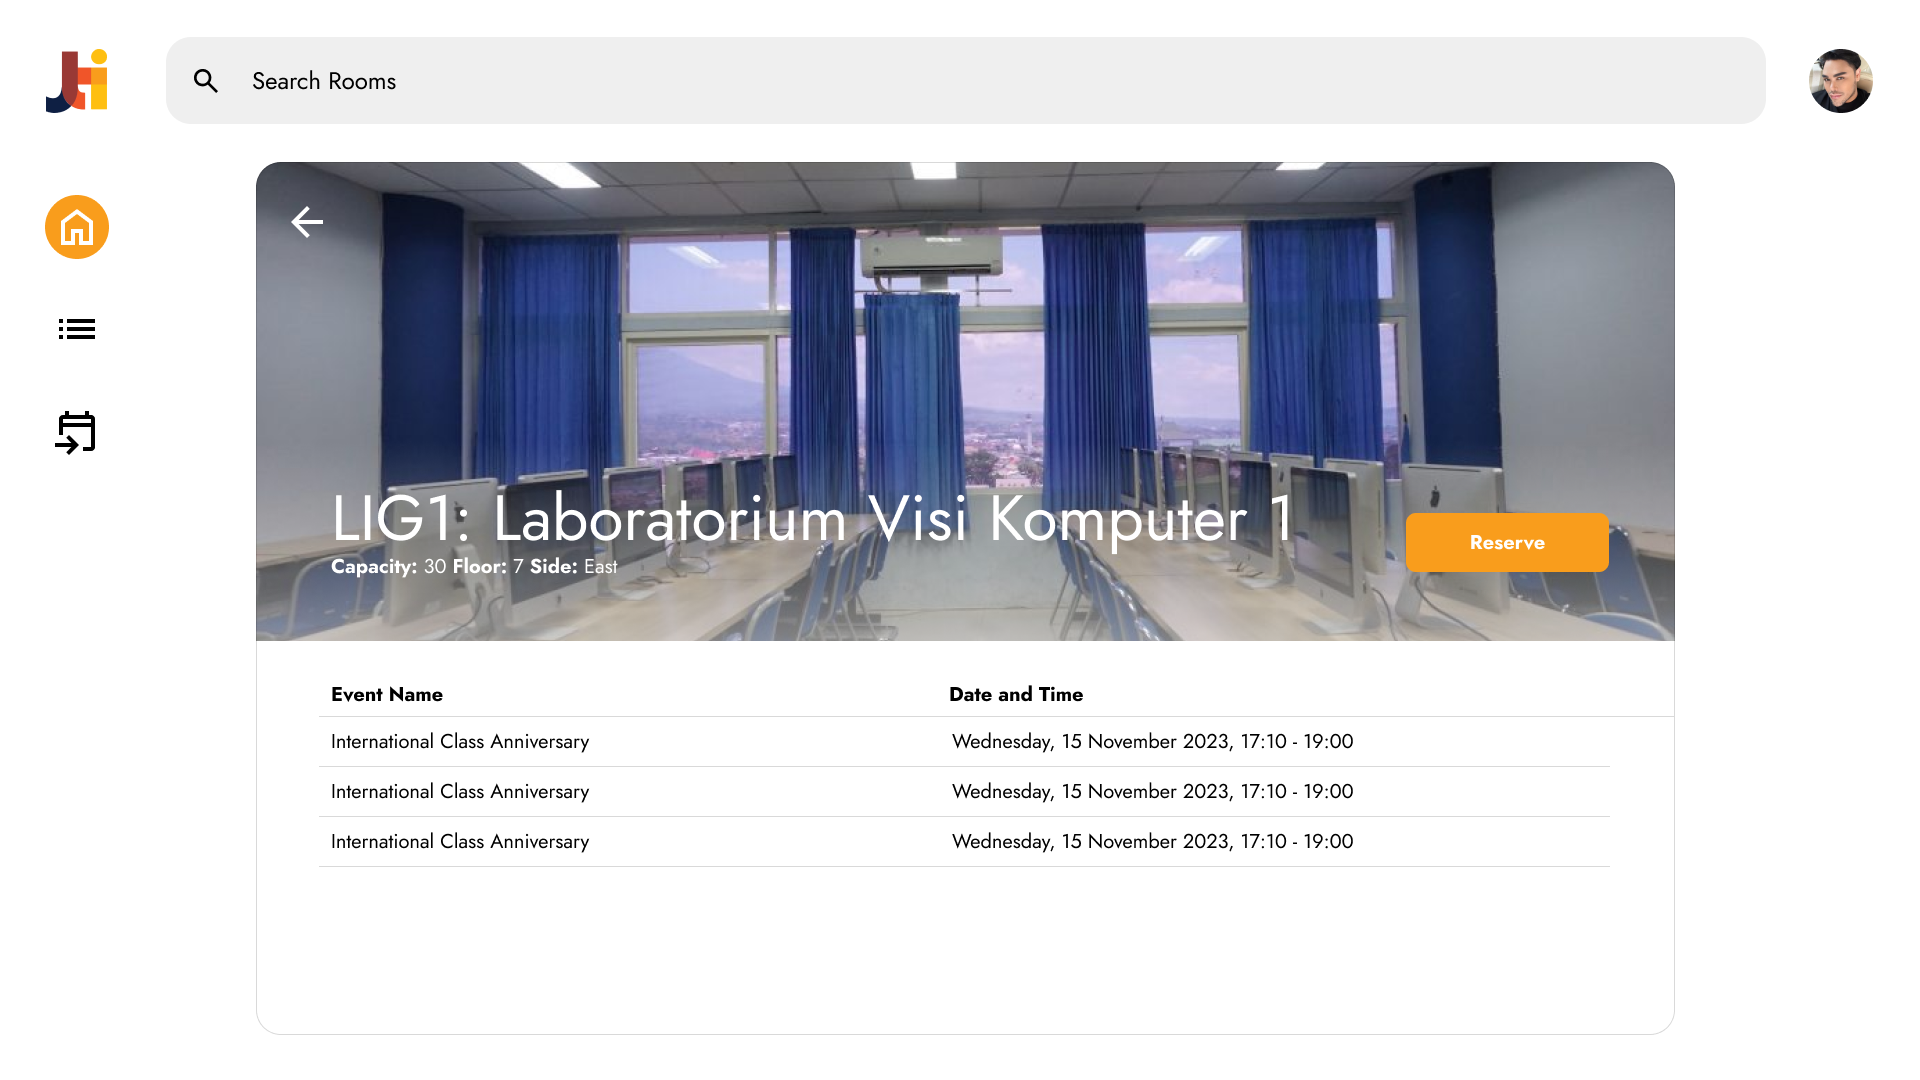
\includegraphics[width=\textwidth]{images/figures/UIUX/daroom.png}\\
    \end{center}
    if user select a room, they will landed to this page, where user can see what event is about to run and a button to reserve the room
    \begin{center}
        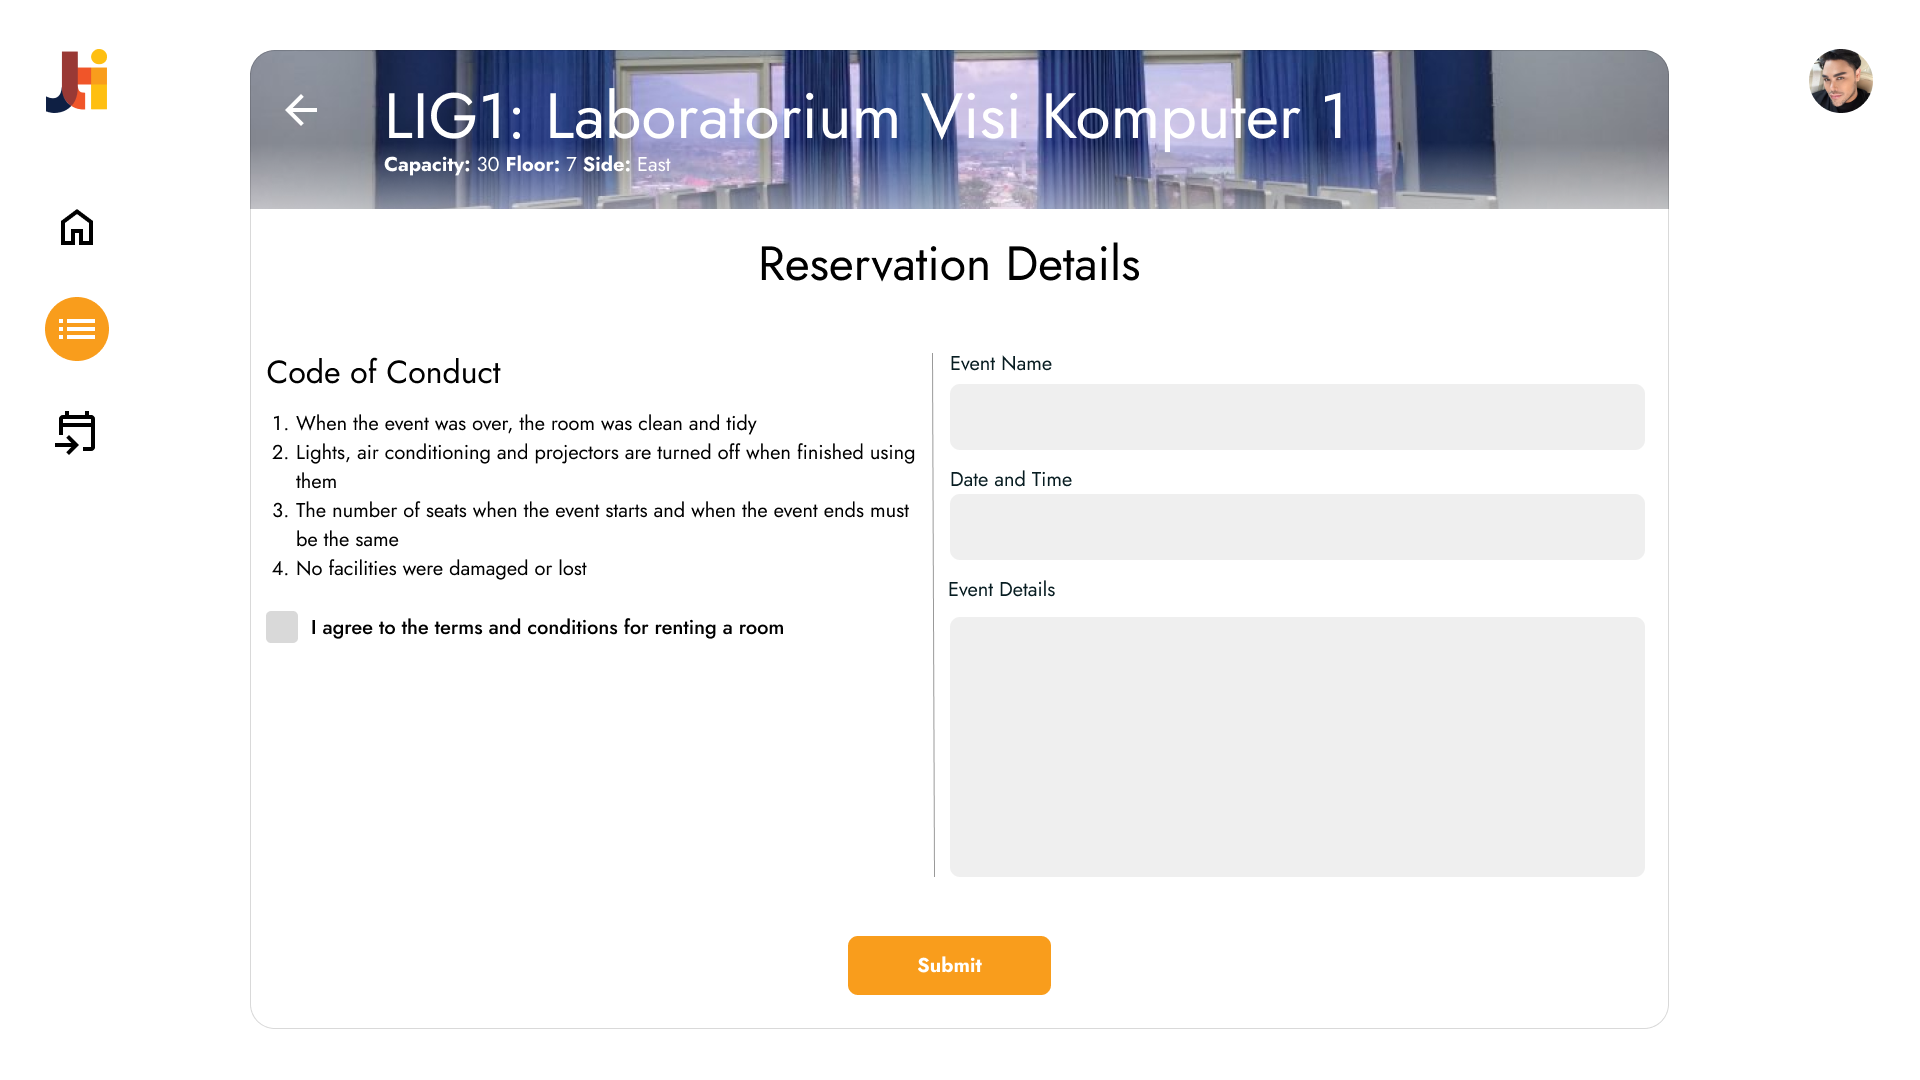
\includegraphics[width=\textwidth]{images/figures/UIUX/reserve_rev.png}\\
    \end{center}
    if user wanted to reserve a room, then user will be directed to this page where user must fill the event name, date and time, and the event details while also agreeing the code of conduct that is provided in the website, after that user can press submit to send the proposal to the admin
    \begin{center}
        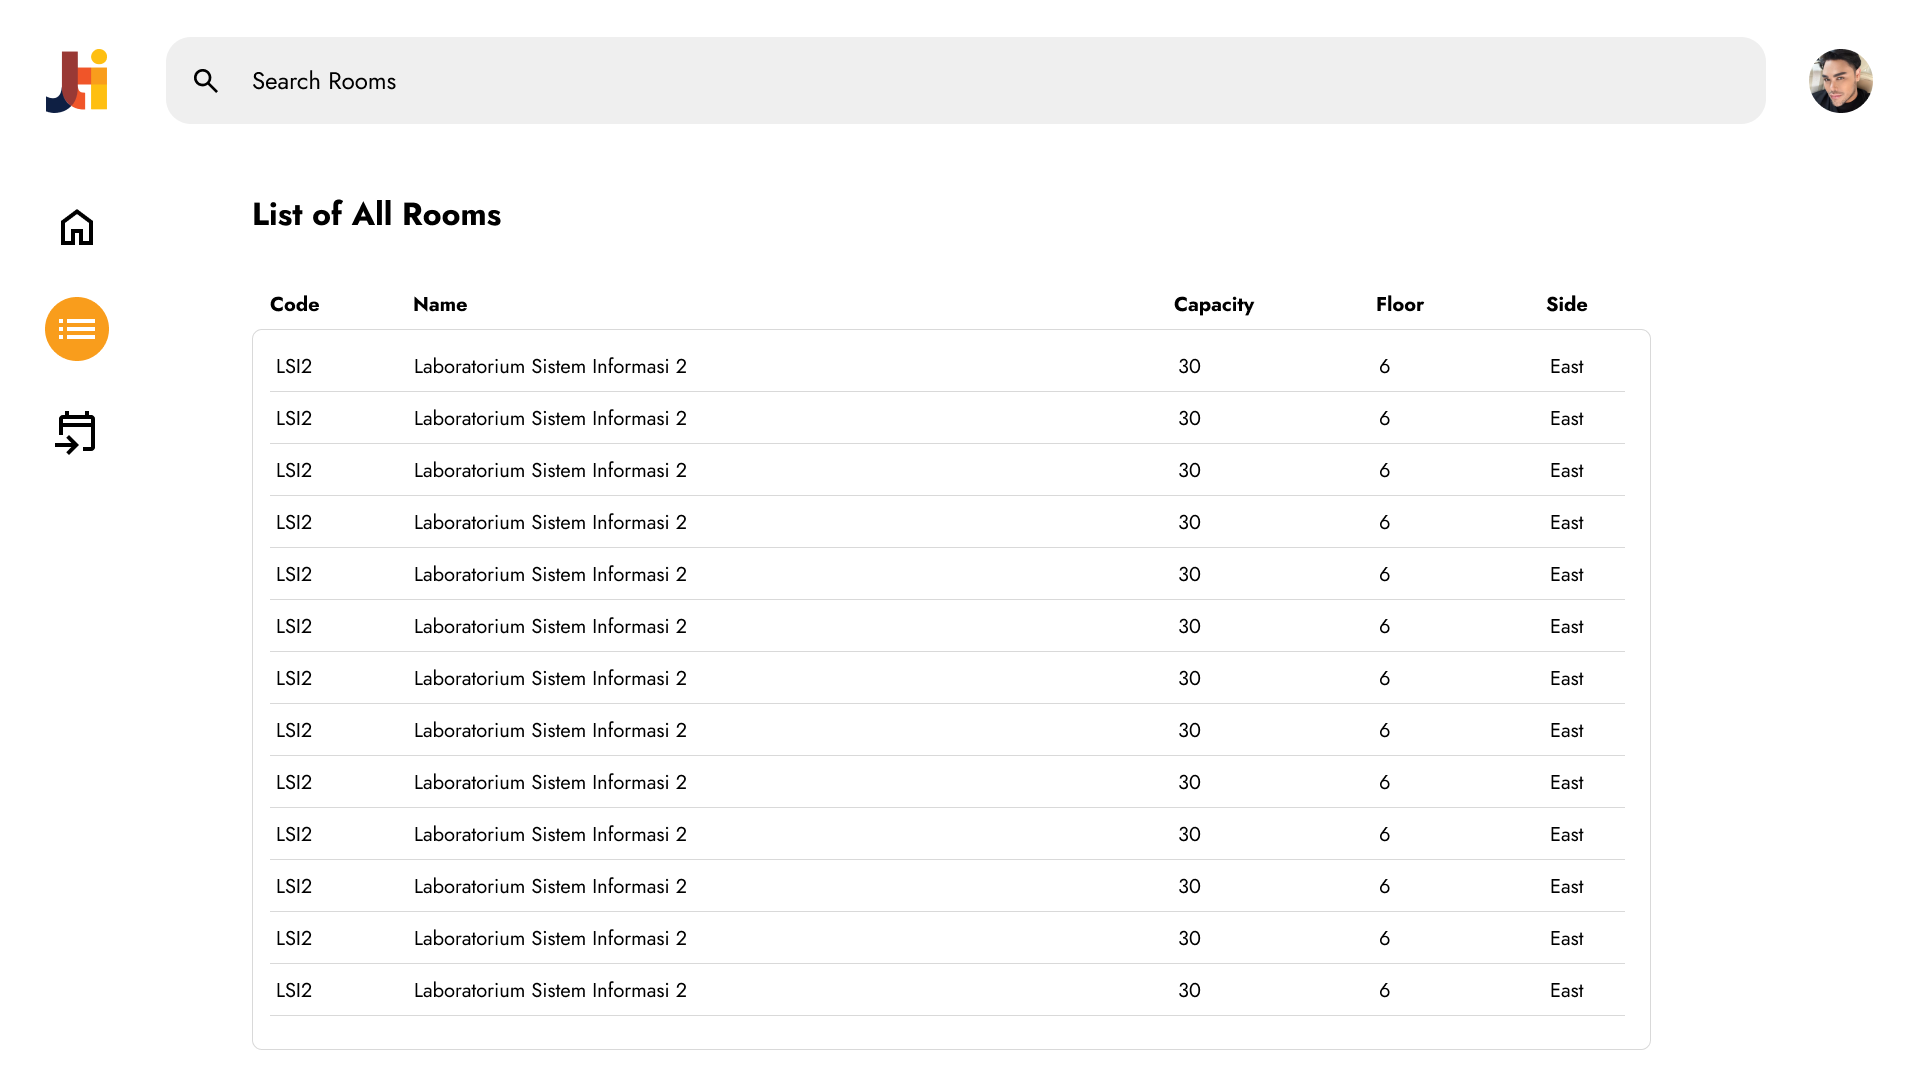
\includegraphics[width=\textwidth]{images/figures/UIUX/list.png}\\
    \end{center}
    user also able to find the list of all room that contains the code, name, capacity, floor, and side of the room itself
    \begin{center}
        \includegraphics[width=\textwidth]{images/figures/UIUX/upcoming.png}\\
    \end{center}
    lastly, user can see what upcoming event, user can see when and where the event will be held
    \newpage
    \subsection{Admin}
    \begin{center}
        \includegraphics[width=\textwidth]{images/figures/UIUX/login.png}\\
    \end{center}
    admin landed in the login screen and login with provided username and password
    \begin{center}
        \includegraphics[width=\textwidth]{images/figures/UIUX/home 1.png}\\
    \end{center}
    upon logged in admin will directed to the homepage where admin can view pending approval and list of approved room
    \begin{center}
        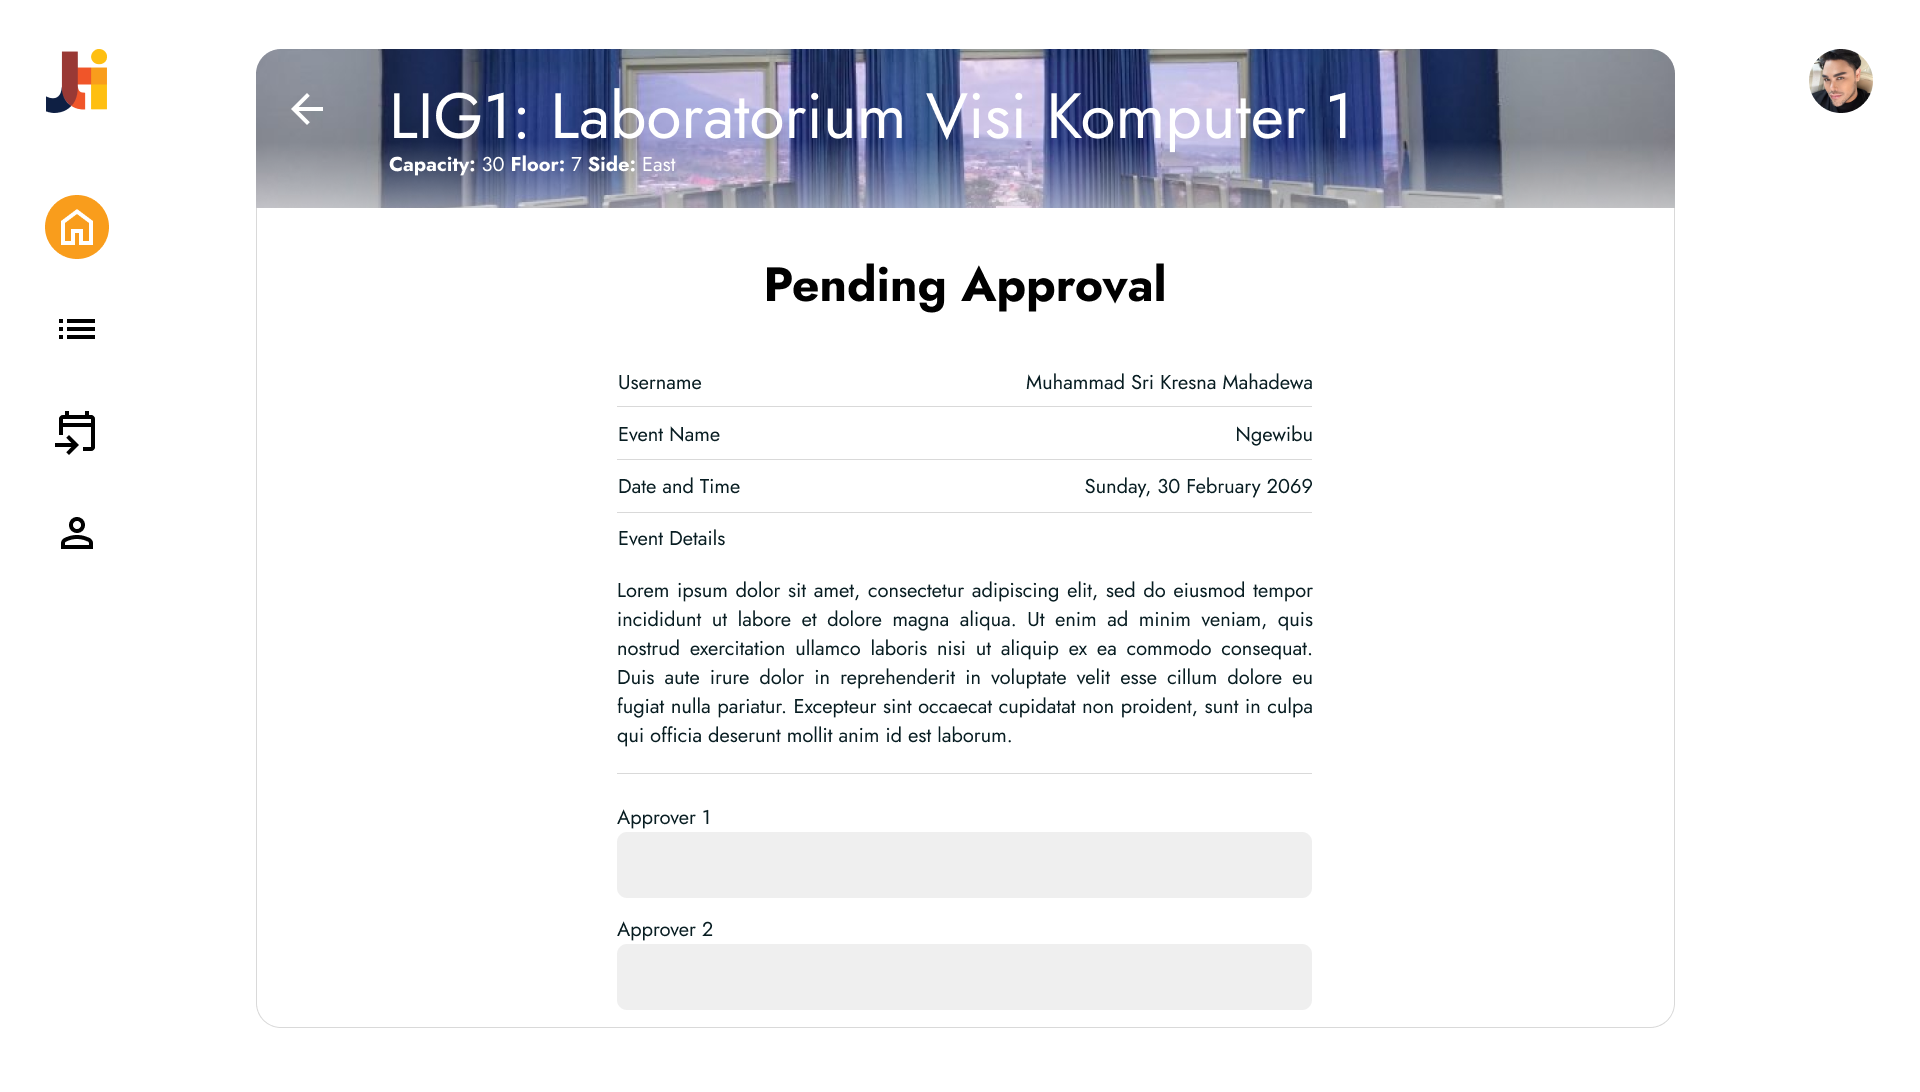
\includegraphics[width=\textwidth]{images/figures/UIUX/approval.png}\\
    \end{center}
    if admin choose pending approval, then admin will see the details of approval, then admin will choose where and who the approval should be given to, since room tenant already has their own terms and service, where it can be changed anytime, we decided to make the approval is determined by the admin so that the user won't be confused where the proposal should be given to, then admin can accept or reject the approval
    \begin{center}
        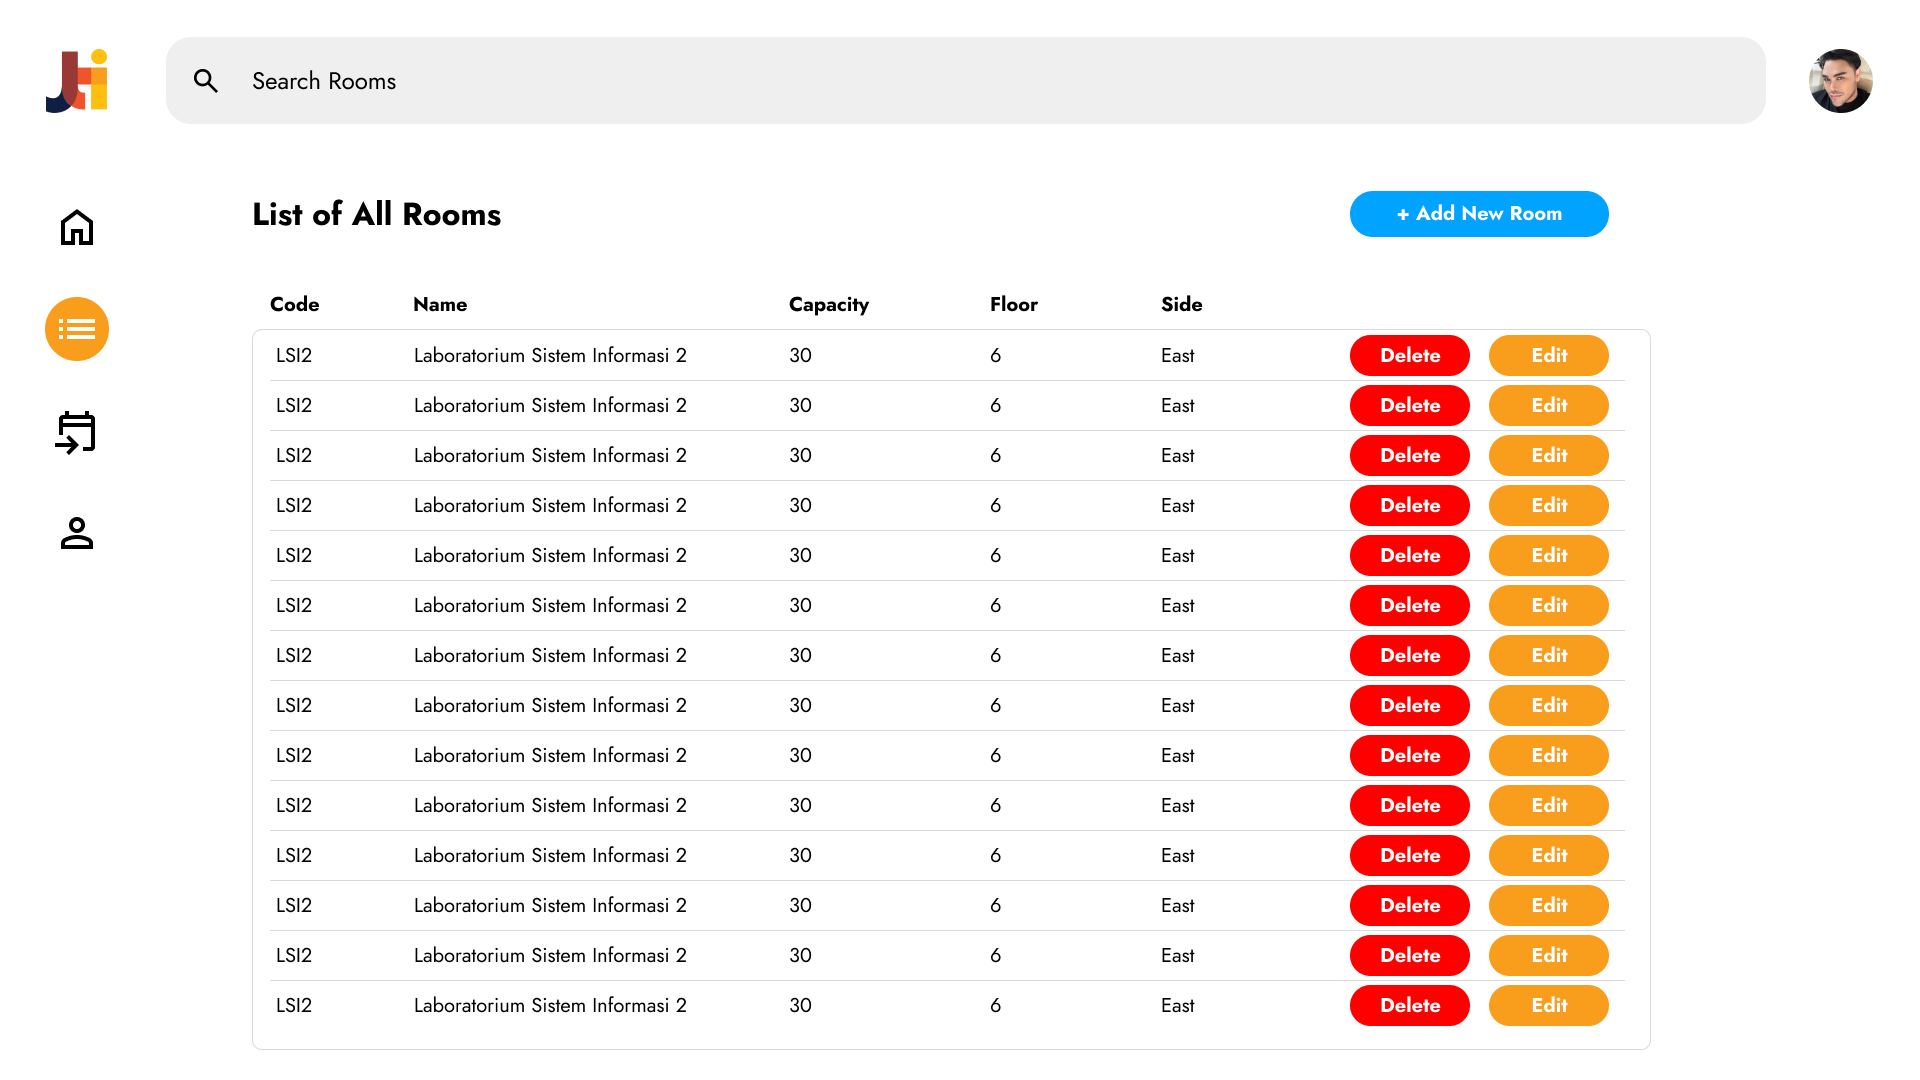
\includegraphics[width=\textwidth]{images/figures/UIUX/list 1.png}\\
    \end{center}
    the next menu is the list of all rooms where admin can create, read, update, delete the room using the provided button
    \begin{center}
        \includegraphics[width=\textwidth]{images/figures/UIUX/add_new_room.png}\\
    \end{center}
    this is the page of adding a new room, admin can fill the room name, room code, floor, side, capacity, and add cover image for the room itself
    \begin{center}
        \includegraphics[width=\textwidth]{images/figures/UIUX/edit_room_details.png}\\
    \end{center}
    on the other page, user can also edit the details of the existing room, containing the same details that is available in the adding new room
    \begin{center}
        \includegraphics[width=\textwidth]{images/figures/UIUX/upcoming 1.png}\\
    \end{center}
    \subsection{Approver}
    \begin{center}
        \includegraphics[width=\textwidth]{images/figures/UIUX/login.png}\\
    \end{center}
    for approver, started from login like usual using provided username and password
    \begin{center}
        \includegraphics[width=\textwidth]{images/figures/UIUX/home 2.png}\\
    \end{center}
    upon landing in the homepage, approver can see list of pending approval
    \begin{center}
        \includegraphics[width=\textwidth]{images/figures/UIUX/approval 1.png}\\
    \end{center}
    if the approver choose a list, they will directed to the approval page, where approver can approve or reject the approval
    \begin{center}
        \includegraphics[width=\textwidth]{images/figures/UIUX/approved.png}\\
    \end{center}
    lastly, approver can see their approved events from the last menu
    \subsection{Prototype Link}
    \noindent
    \resizebox{.5\textwidth}{!}{
        \begin{tabular}{l l}
            User & : \url{https://s.id/1YKyu}\\
            Admin & : \url{https://s.id/1YKyD}\\
            Approver & : \url{https://s.id/1YKyH}\\
        \end{tabular}
    }
% \chapter{Software Testing Document}
%     \section{Blackbox Test Result}
%     \section{Quality Test Result}
\end{document}